\section{Các thí nghiệm chuyên sâu}
\label{sec:tn}

\subsection{Thiết lập các thí nghiệm}
\label{sec:tn-thiet-lap}

Trên dữ liệu chuẩn, PatchCore đã đạt image-AUROC trên 0,95 ở hầu hết các loại, nên con số này không còn phân biệt
được các phương pháp. Câu hỏi thực tế hơn là khi điều kiện nhà máy khác với giả định của bộ dữ liệu, phương pháp nào
hỏng trước, hỏng theo cách nào, và có đoán trước được từ cơ chế của nó không. Mỗi phương pháp có một giả định ngầm
riêng: Autoencoder giả định lỗi khó tái tạo hơn vùng bình thường; PaDiM giả định ảnh đã căn chỉnh và tại mỗi vị trí
chỉ có một kiểu bình thường; PatchCore giả định mọi patch bình thường đều đã có một patch gần nó trong bộ nhớ.

Từ đó nhóm đặt năm câu hỏi, ứng với năm thí nghiệm. Thí nghiệm 1 hỏi phương pháp nào suy giảm khi tập huấn luyện lẫn
ảnh lỗi. Thí nghiệm 2 hỏi phương pháp nào mất khả năng phát hiện nhanh hơn khi chỉ có 1 đến 16 ảnh tốt. Thí nghiệm 3
hỏi mô hình học trên một loại sản phẩm dùng được cho loại khác tới đâu, và cần bao nhiêu ảnh của loại mới để thích
nghi. Thí nghiệm 4 hỏi phương pháp nào nhầm thay đổi điều kiện chụp với lỗi thật nhiều hơn. Thí nghiệm 5 hỏi các thất
bại cụ thể có đoán trước được từ cơ chế hay không.

Các thí nghiệm dùng grid, screw, transistor của MVTec AD, hai loại của MVTec AD 2 và bốn loại pcb của VisA, với đúng
cấu hình ở Bảng~\ref{tab:hyper} và ngưỡng ở Mục~\ref{sec:dat-nguong}. Thí nghiệm 1, 2 và 5 so với một mốc huấn luyện
trên toàn bộ \texttt{train/good} (Bảng~\ref{tab:tn-moc}), khác với mốc 9 loại ở Mục~\ref{sec:ket-qua-tong-hop} vốn tách
15\% ảnh để đặt ngưỡng, nên các số liệu có chênh lệch nhỏ. Chênh lệch lớn nhất là ở Autoencoder (ví dụ transistor 0,753
so với 0,786), cũng là phương pháp dao động nhiều nhất giữa các lần chạy (Mục~\ref{sec:tn1}). Thí nghiệm 1 lặp 5 seed,
Thí nghiệm 2 lặp 3 seed, các thí nghiệm còn lại chạy một lần. Tất cả chạy trên Google Colab; một phần của Thí nghiệm 4
chạy trên CPU khi hết hạn mức GPU.

\begin{table}[htbp]
  \centering
  \caption{Image-AUROC của mốc huấn luyện trên toàn bộ \texttt{train/good}}
  \label{tab:tn-moc}
  \begin{tabular}{@{}lccc@{}}
    \toprule
    Loại & Autoencoder & PaDiM & PatchCore \\
    \midrule
    grid       & 0,825 & 0,934 & 0,989 \\
    screw      & 0,787 & 0,722 & 0,955 \\
    transistor & 0,753 & 0,968 & 0,999 \\
    \bottomrule
  \end{tabular}
\end{table}

\subsection{Thí nghiệm 1: dữ liệu huấn luyện lẫn ảnh lỗi}
\label{sec:tn1}

Trong nhà máy, tập ảnh tốt thường được thu tự động và có thể lẫn một ít sản phẩm lỗi chưa được phát hiện. Mỗi phương
pháp có một cách hỏng dự kiến. Autoencoder có thể học luôn cách tái tạo lỗi, nên sai số trên lỗi thật giảm. Với PaDiM,
trung bình dịch về phía lỗi và hiệp phương sai phình ra, nên khoảng cách Mahalanobis của lỗi nhỏ lại. PatchCore ghi
patch lỗi vào bộ nhớ, nên lỗi cùng kiểu ở tập test tìm được láng giềng rất gần và có điểm thấp.

Nhóm trộn 0\%, 5\%, 10\% và 20\% ảnh lỗi vào tập huấn luyện của screw và grid; ảnh lỗi lấy từ tập test rồi bị loại
khỏi tập đánh giá, mỗi mức lặp 5 seed. Grid chỉ có 57 ảnh lỗi nên dừng ở 10\% (29 ảnh); số ảnh lỗi trộn vào screw ở
ba mức là 17, 36 và 80.

\begin{table}[htbp]
  \centering
  \caption{Image-AUROC theo tỷ lệ ảnh lỗi trong tập huấn luyện (trung bình 5 seed)}
  \label{tab:tn1}
  \begin{tabular}{@{}llccccc@{}}
    \toprule
    Loại & Phương pháp & 0\% & 5\% & 10\% & 20\% & Chênh lệch \\
    \midrule
    screw & Autoencoder & 0,745 & 0,720 & 0,682 & 0,689 & $-0{,}056$ \\
          & PaDiM       & 0,737 & 0,740 & 0,732 & 0,721 & $-0{,}016$ \\
          & PatchCore   & 0,955 & 0,945 & 0,930 & 0,921 & $-0{,}034$ \\
    \midrule
    grid  & Autoencoder & 0,860 & 0,851 & 0,853 & -- & $\approx 0$ \\
          & PaDiM       & 0,944 & 0,946 & 0,946 & -- & $\approx 0$ \\
          & PatchCore   & 0,993 & 0,995 & 0,995 & -- & $\approx 0$ \\
    \bottomrule
  \end{tabular}
\end{table}

\begin{figure}[htbp]
  \centering
  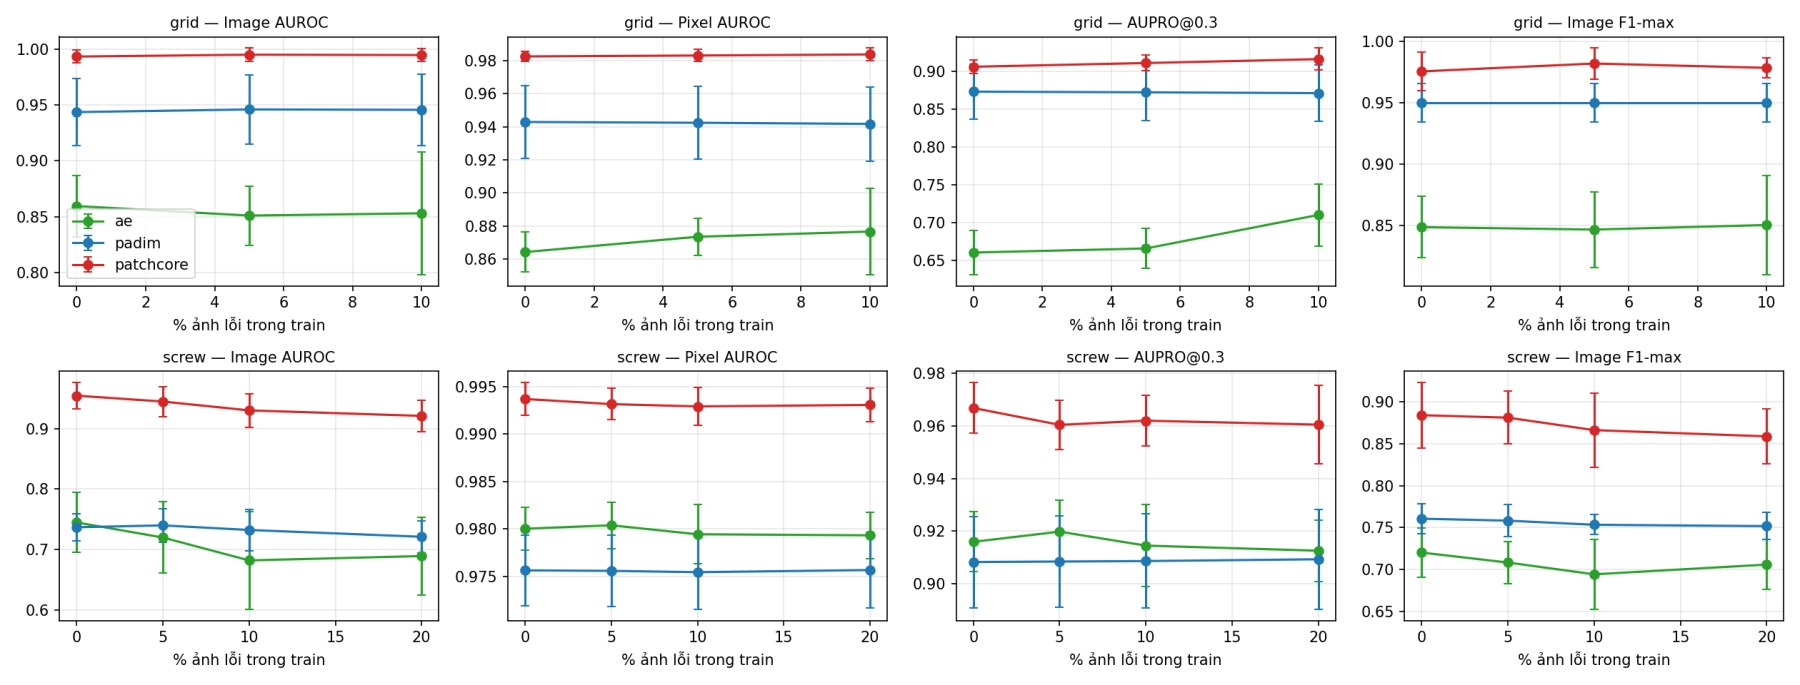
\includegraphics[width=\linewidth]{images/tn/tn1_nhiem_ban.jpg}
  \caption[I-AUROC và AUPRO theo tỷ lệ ảnh lỗi trong tập huấn luyện]{I-AUROC và AUPRO theo tỷ lệ ảnh lỗi trong tập
    huấn luyện trên screw và grid (trung bình 5 seed, thanh lỗi là độ lệch chuẩn)}
  \label{fig:tn1}
\end{figure}

Không phương pháp nào sụp đổ khi tập huấn luyện lẫn tới 20\% ảnh lỗi (Bảng~\ref{tab:tn1}, Hình~\ref{fig:tn1}). Mức
suy giảm lớn nhất chỉ 3 đến 6 điểm image-AUROC và chỉ xuất hiện trên screw; trên grid cả ba gần như không đổi. Lỗi
trên grid là vùng nhỏ trên một bề mặt lặp lại, nên vài ảnh lỗi chỉ thêm một lượng rất nhỏ patch bất thường vào hàng
chục nghìn patch tốt, không đủ để kéo lệch phân phối Gauss hay chiếm bộ nhớ.

Hình dạng đường suy giảm khớp với cơ chế. PatchCore giảm gần tuyến tính và nhất quán, cả 5 seed đều giảm trên screw:
mỗi ảnh lỗi thêm vào là thêm một số patch lỗi vào bộ nhớ, nên ảnh hưởng cộng dồn theo số ảnh. PaDiM phẳng tới 10\% và
chỉ giảm nhẹ ở 20\%, vì phân phối Gauss là thống kê trung bình trên hàng trăm ảnh nên vài ảnh lỗi bị pha loãng.
Autoencoder giảm ở 5--10\% rồi đi ngang, nhưng 2 trong 5 seed lại tăng image-AUROC, nên không kết luận được đây là hiệu
ứng thật hay dao động của quá trình huấn luyện.

Khả năng định vị gần như không đổi: trên screw, AUPRO thay đổi $-0{,}006$ với PatchCore, gần 0 với PaDiM và $-0{,}003$
với Autoencoder, còn pixel-AUROC thay đổi khoảng $-0{,}001$. Dữ liệu bẩn làm hỏng khả năng xếp hạng ảnh, vốn dựa vào
giá trị lớn nhất của bản đồ và rất nhạy với vài patch, nhưng không làm hỏng hình dạng bản đồ. Riêng AUPRO của
Autoencoder trên grid còn tăng từ 0,660 lên 0,710 ở mức 10\%; nhóm chưa có thí nghiệm để giải thích hiện tượng này.

Độ lệch chuẩn image-AUROC giữa 5 seed là 0,064 (screw) và 0,036 (grid) với Autoencoder, 0,028 và 0,031 với PaDiM,
0,025 và 0,006 với PatchCore. Trên screw, Autoencoder dao động gấp 2 đến 3 lần hai phương pháp còn lại; trên grid
nó chỉ ngang PaDiM nhưng gấp 6 lần PatchCore. Lý do là ngoài việc chọn ảnh lỗi nào được trộn vào, mạng còn được huấn
luyện từ khởi tạo ngẫu nhiên. Trên screw, độ dao động này còn lớn hơn chính mức
suy giảm do dữ liệu bẩn (0,056); với Autoencoder, seed ảnh hưởng tới kết quả nhiều hơn việc làm sạch dữ liệu.

Như vậy cả ba phương pháp đều khá bền với 5--20\% dữ liệu bẩn. PatchCore suy giảm đều theo số ảnh lỗi nhưng vẫn tốt
nhất về giá trị tuyệt đối: 0,921 ở mức 20\% vẫn cao hơn PaDiM trên dữ liệu sạch (0,737).

\subsection{Thí nghiệm 2: chỉ có vài ảnh tốt}
\label{sec:tn2}

Khi một dây chuyền mới chỉ có vài ảnh sản phẩm tốt, ba cách học phản ứng khác nhau. PaDiM phải ước lượng trung bình
và ma trận hiệp phương sai $100\times100$ tại mỗi vị trí; với ít ảnh, ma trận gần suy biến và chỉ còn nhờ thành phần
$0{,}01\,I$, nên khoảng cách Mahalanobis gần như thành khoảng cách Euclid tới trung bình. PatchCore không cần ước lượng
thống kê và mỗi ảnh vẫn cho hàng nghìn patch, nhưng bộ nhớ chỉ bao phủ những biến thể đã thấy. Autoencoder cần đủ dữ
liệu để học cấu trúc chung; với vài ảnh, nó dễ học thuộc hoặc dựng ra ảnh mờ.

Với mỗi loại, nhóm chọn ngẫu nhiên $k \in \{1, 2, 4, 8, 16\}$ ảnh tốt từ tập huấn luyện (3 seed), xây dựng mô hình rồi
đánh giá trên toàn bộ tập test, và so với mốc ở Bảng~\ref{tab:tn-moc}.

\begin{table}[htbp]
  \centering
  \caption[I-AUROC và AUPRO theo số ảnh huấn luyện $k$]{I-AUROC và AUPRO theo số ảnh huấn luyện $k$ (trung bình 3
    seed; ``đủ'' là mốc dùng toàn bộ tập huấn luyện)}
  \label{tab:tn2}
  \small
  \begin{tabular}{@{}llcccccc@{}}
    \toprule
    & & \multicolumn{3}{c}{Image-AUROC} & \multicolumn{3}{c}{AUPRO} \\
    \cmidrule(lr){3-5}\cmidrule(l){6-8}
    Loại & Phương pháp & đủ & $k = 16$ & $k = 1$ & đủ & $k = 16$ & $k = 1$ \\
    \midrule
    grid       & Autoencoder & 0,825 & 0,630 & 0,611 & 0,658 & 0,244 & 0,253 \\
               & PaDiM       & 0,934 & 0,759 & 0,586 & 0,872 & 0,717 & 0,416 \\
               & PatchCore   & 0,989 & 0,794 & 0,597 & 0,900 & 0,502 & 0,276 \\
    \midrule
    screw      & Autoencoder & 0,787 & 0,468 & 0,305 & 0,908 & 0,736 & 0,658 \\
               & PaDiM       & 0,722 & 0,532 & 0,535 & 0,890 & 0,818 & 0,604 \\
               & PatchCore   & 0,955 & 0,634 & 0,448 & 0,951 & 0,844 & 0,666 \\
    \midrule
    transistor & Autoencoder & 0,753 & 0,660 & 0,621 & 0,709 & 0,561 & 0,252 \\
               & PaDiM       & 0,968 & 0,914 & 0,568 & 0,929 & 0,903 & 0,576 \\
               & PatchCore   & 0,999 & 0,995 & 0,827 & 0,952 & 0,931 & 0,806 \\
    \bottomrule
  \end{tabular}
\end{table}

\begin{figure}[htbp]
  \centering
  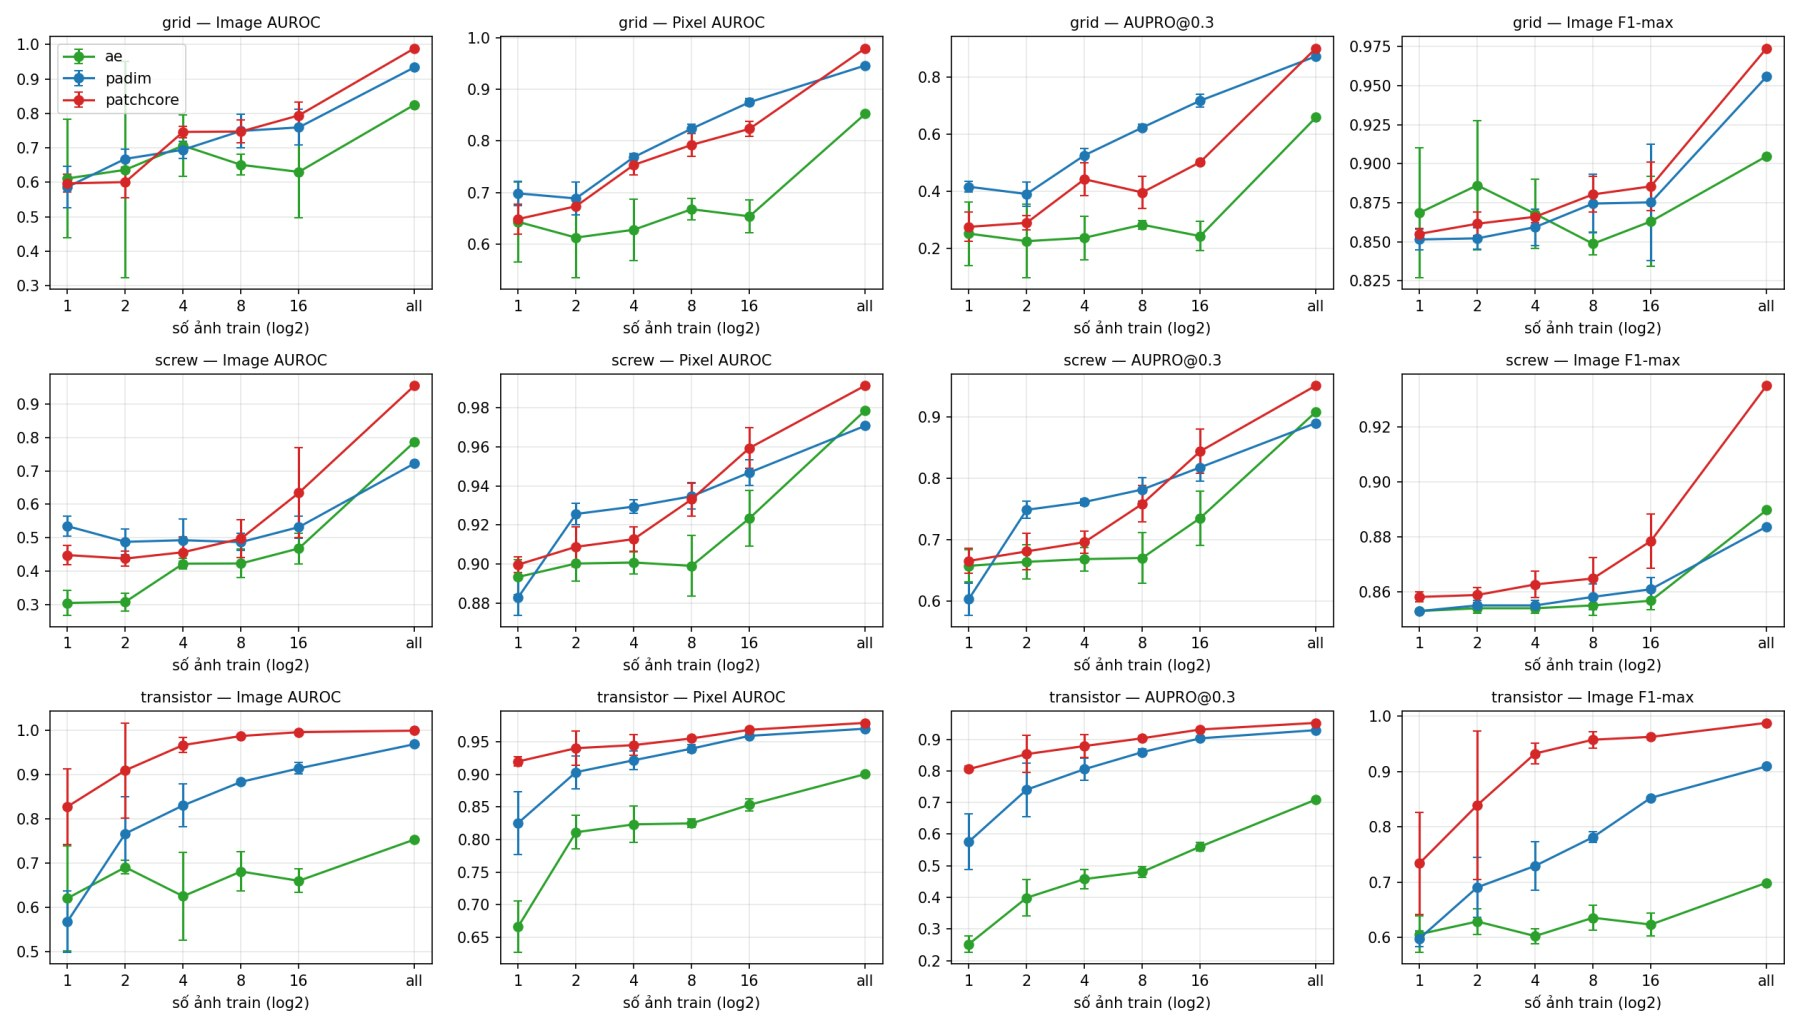
\includegraphics[width=\linewidth]{images/tn/tn2_few_shot.jpg}
  \caption[I-AUROC và AUPRO theo số ảnh huấn luyện]{I-AUROC và AUPRO theo số ảnh huấn luyện $k$ cho grid, screw,
    transistor (trung bình 3 seed; đường ngang là mốc dùng toàn bộ tập huấn luyện)}
  \label{fig:tn2}
\end{figure}

Phương pháp nào mất khả năng phát hiện nhanh hơn phụ thuộc mạnh vào loại sản phẩm (Bảng~\ref{tab:tn2},
Hình~\ref{fig:tn2}). Với transistor, vật thể cố định và ảnh được căn chỉnh tốt, PatchCore gần như không mất gì: còn
0,995 với 16 ảnh, đạt 0,966 với 4 ảnh và vẫn 0,827 với 1 ảnh. PaDiM giữ được tới 16 ảnh (0,914) nhưng rơi về 0,568 khi
chỉ có 1 ảnh, đúng dự đoán vì một ảnh không đủ để ước lượng phân phối. Với grid, cả ba giảm về khoảng 0,6 khi chỉ có
1 ảnh, dù một ảnh grid đã chứa rất nhiều patch lặp lại; khả năng là lưới trong MVTec AD thay đổi góc và tỷ lệ giữa các
ảnh, nên vài ảnh không bao phủ hết các biến thể. Với screw, cả ba ở gần hoặc dưới mức ngẫu nhiên cho tới 8 ảnh.
Autoencoder với 1 ảnh chỉ còn 0,305, tức xếp hạng ngược: ảnh tốt bị chấm điểm cao hơn ảnh lỗi. Một mô hình dưới 0,5
không chỉ yếu mà đang phản ứng với một tín hiệu khác với lỗi; Mục~\ref{sec:tn2b} tìm tín hiệu đó.

Phát hiện và định vị không suy giảm cùng nhịp, và thứ tự phụ thuộc vào loại. Trên screw, AUPRO giảm chậm hơn
image-AUROC ở cả ba phương pháp: với 16 ảnh, PatchCore chỉ còn image-AUROC 0,634 nhưng AUPRO vẫn 0,844. Mô hình vẫn
thấy vùng lỗi sáng lên trong ảnh lỗi, nhưng ảnh tốt cũng có những vùng sáng khác do góc xoay chưa gặp, nên giá trị lớn
nhất của ảnh không còn phân biệt được. Trên grid thì ngược lại: với 16 ảnh, AUPRO của PatchCore giảm từ 0,900 xuống
0,502 và của Autoencoder từ 0,658 xuống 0,244, gấp đôi mức giảm image-AUROC, vì vài ảnh không bao phủ hết biến thể của
lưới nên bản đồ sáng cả ở vùng tốt quanh vết lỗi. PaDiM giữ AUPRO trên grid tốt hơn PatchCore rõ rệt (0,717 so với
0,502): cách học theo vị trí có lợi khi bề mặt đồng nhất. Trên transistor, cả hai chỉ số của PatchCore và PaDiM gần
như không đổi tới 16 ảnh, còn Autoencoder mất khả năng định vị nhanh hơn khả năng phát hiện.

Thứ hạng của ba phương pháp không nhất quán giữa các loại. Điều quyết định không phải bản thân số ảnh, mà là $k$ ảnh
đó có bao phủ được biến thiên tự nhiên của ảnh tốt (góc, vị trí, ánh sáng) hay không. Với transistor, vật thể cố
định và ảnh gần như giống hệt nhau, PatchCore chỉ cần 4 ảnh; grid tuy không xoay nhưng lưới thay đổi giữa các ảnh, nên
16 ảnh vẫn chưa đủ (0,794); với screw xoay tự do, cả ba phương pháp vẫn dưới 0,64 ở 16 ảnh, tức không dùng được trong
khoảng số ảnh đã thử.

\subsubsection{Vì sao screw thất bại khi có ít ảnh}
\label{sec:tn2b}

Image-AUROC dưới 0,5 trên screw gợi ý mô hình đang chấm điểm theo một yếu tố không liên quan tới lỗi. Nhóm kiểm tra
hai ứng viên: góc xoay của con vít và độ sáng của ảnh.

Góc của mỗi con vít được ước lượng từ trục chính của vùng tối là thân vít (Hình~\ref{fig:tn2b-goc}). Với mỗi ảnh test,
nhóm tính khoảng cách góc tới ảnh huấn luyện gần nhất, rồi đo tương quan Spearman giữa khoảng cách này và điểm bất
thường (Hình~\ref{fig:tn2b-diem}). Tương quan là 0,82 đến 0,92 với PatchCore (4 và 8 ảnh) và 0,38 đến 0,60 với PaDiM:
với PatchCore, góc xoay giải thích gần như toàn bộ thứ hạng điểm. Trong khi đó, khoảng cách góc trung bình của ảnh tốt
và ảnh lỗi gần như bằng nhau (35,1° so với 33,4° với 4 ảnh), nên điểm bị chi phối bởi một yếu tố không phân biệt
tốt với lỗi, và image-AUROC xoay quanh 0,5.

\begin{figure}[htbp]
  \centering
  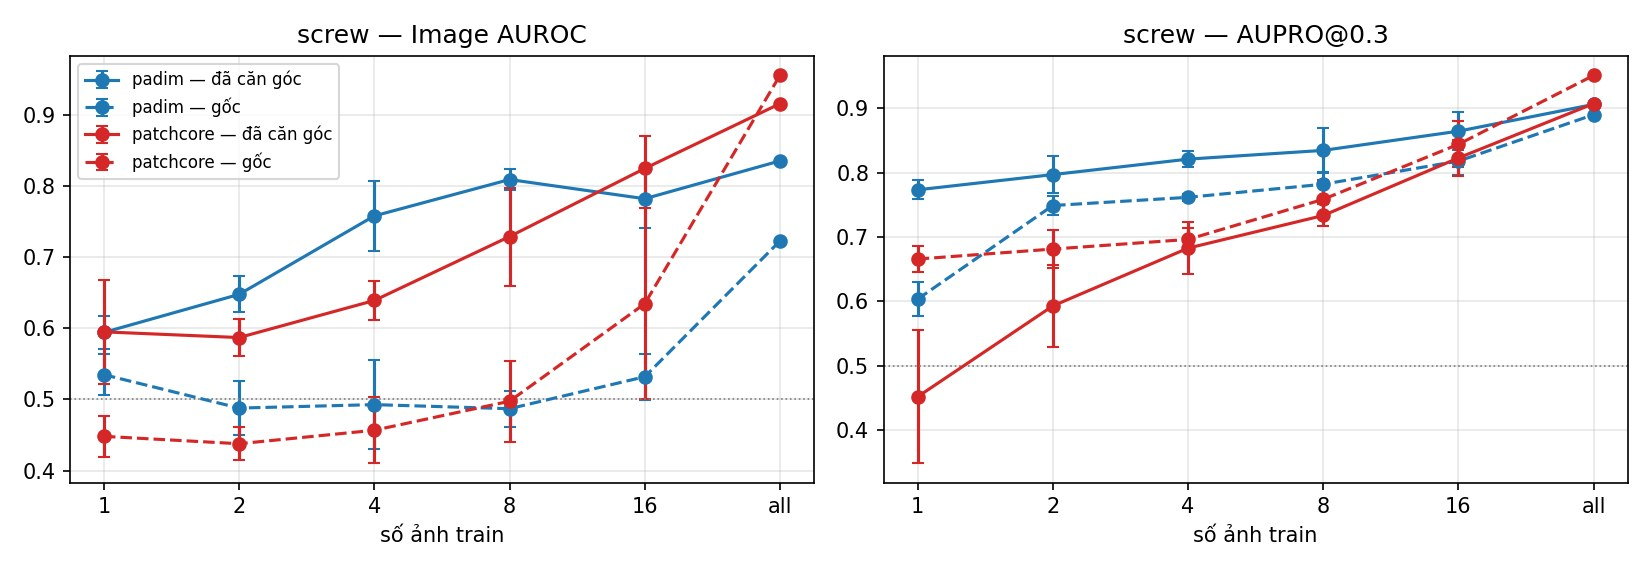
\includegraphics[width=\linewidth]{images/tn/tn2b_goc_xoay_vi_du.jpg}
  \caption{Ảnh screw tốt ở nhiều góc xoay khác nhau, kèm góc ước lượng}
  \label{fig:tn2b-goc}
\end{figure}

\begin{figure}[htbp]
  \centering
  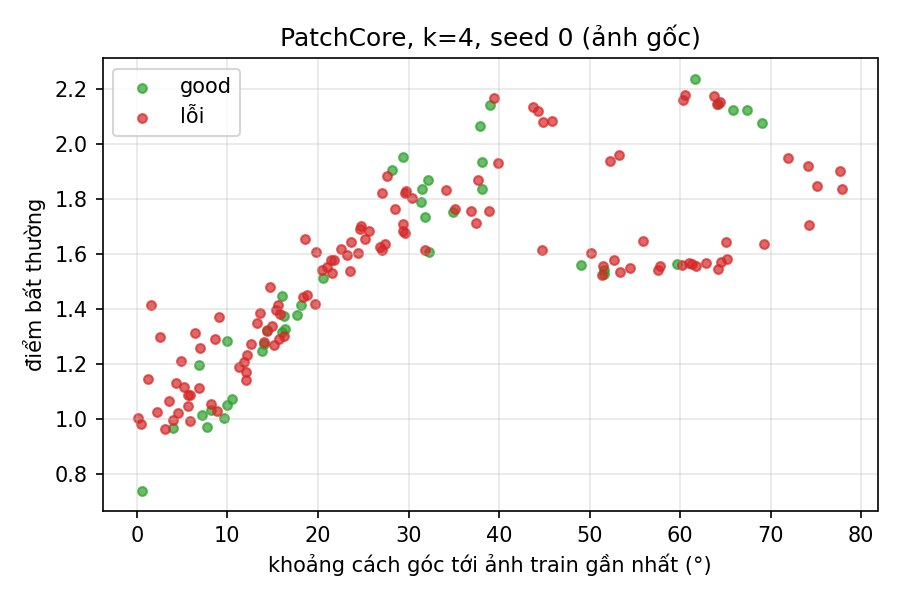
\includegraphics[width=0.7\linewidth]{images/tn/tn2b_diem_theo_goc.jpg}
  \caption{Điểm bất thường theo khoảng cách góc tới ảnh huấn luyện gần nhất}
  \label{fig:tn2b-diem}
\end{figure}

Để kiểm chứng, nhóm xoay mọi ảnh, cả huấn luyện và test, về cùng một hướng trước khi xây dựng mô hình
(Bảng~\ref{tab:tn2b}, Hình~\ref{fig:tn2b-can-chinh}). Căn chỉnh tăng image-AUROC 19 đến 32 điểm khi có ít ảnh, và tăng
11 điểm cho PaDiM khi dùng toàn bộ tập huấn luyện, xác nhận góc xoay là nguyên nhân chính. Riêng PatchCore với toàn
bộ tập huấn luyện giảm nhẹ từ 0,955 xuống 0,915, chủ yếu do kiểu lỗi thread\_side giảm từ 0,917 xuống 0,795: khi đủ
ảnh, bộ nhớ đã tự bao phủ mọi góc, còn phép xoay với nội suy lại làm mờ chi tiết ren nhỏ.

\begin{table}[htbp]
  \centering
  \caption{Image-AUROC trên screw trước và sau khi căn chỉnh góc}
  \label{tab:tn2b}
  \begin{tabular}{@{}lcc@{}}
    \toprule
    Cấu hình & Trước căn chỉnh & Sau căn chỉnh \\
    \midrule
    PaDiM, 4 ảnh                       & 0,493 & 0,758 \\
    PaDiM, 8 ảnh                       & 0,487 & 0,809 \\
    PatchCore, 8 ảnh                   & 0,497 & 0,729 \\
    PatchCore, 16 ảnh                  & 0,634 & 0,824 \\
    PaDiM, toàn bộ tập huấn luyện      & 0,722 & 0,835 \\
    PatchCore, toàn bộ tập huấn luyện  & 0,955 & 0,915 \\
    \bottomrule
  \end{tabular}
\end{table}

\begin{figure}[htbp]
  \centering
  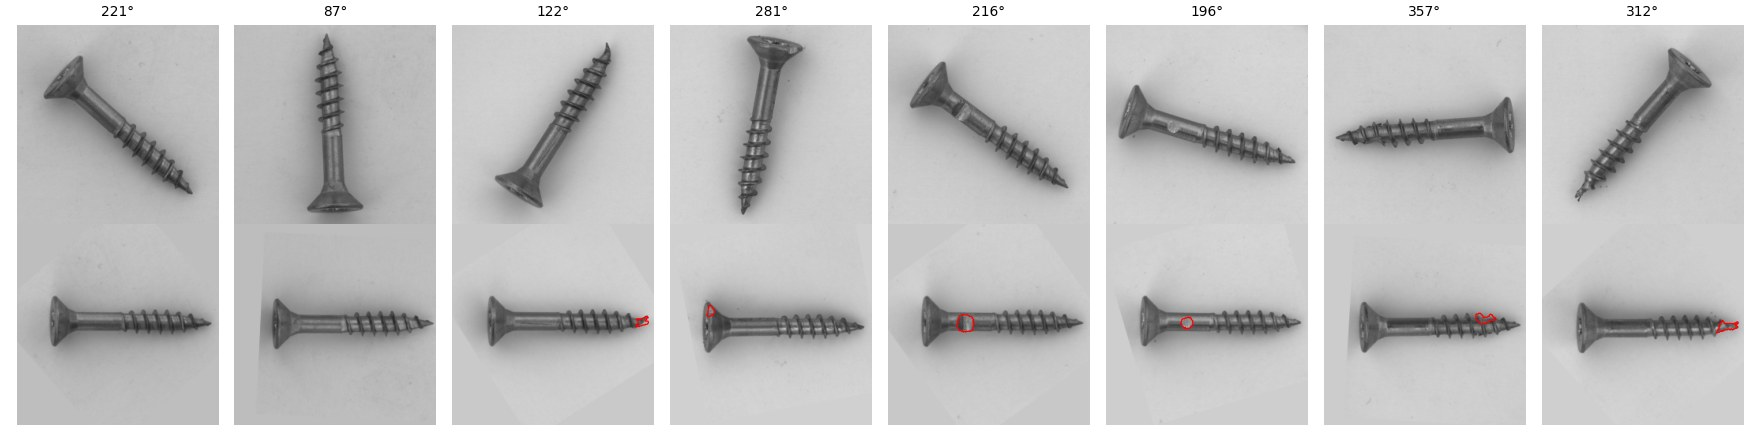
\includegraphics[width=\linewidth]{images/tn/tn2b_can_chinh.jpg}
  \caption{Image-AUROC trước và sau khi căn chỉnh góc trên screw}
  \label{fig:tn2b-can-chinh}
\end{figure}

Khi kiểm tra độ sáng, nhóm phát hiện một độ lệch có hệ thống trong dữ liệu (Bảng~\ref{tab:tn2b-sang}): ảnh test tốt
của screw tối hơn rõ rệt so với cả ảnh huấn luyện lẫn ảnh lỗi. Chỉ dùng độ sáng trung bình làm điểm bất thường đã đạt
AUROC bằng 1,0 trên 86 ảnh kiểm tra (41 ảnh tốt và 45 trong số 119 ảnh lỗi). Một mô hình nhạy với độ sáng vì vậy thấy
ảnh test tốt ``lạ'' hơn ảnh lỗi và cho image-AUROC dưới 0,5; đây là lời giải thích cho Autoencoder với 1 ảnh chỉ đạt
0,305 trên screw. Ngược lại, một mô hình cũng có thể đạt điểm cao trên screw mà không thực sự thấy lỗi; hiện tượng này
xuất hiện lại ở Thí nghiệm 3 và 4.

\begin{table}[htbp]
  \centering
  \caption{Độ sáng trung bình (thang 0--255) của các tập ảnh screw}
  \label{tab:tn2b-sang}
  \begin{tabular}{@{}lcc@{}}
    \toprule
    Tập ảnh & Toàn ảnh & Vùng nền \\
    \midrule
    \texttt{train/good}       & 187,5 & 208,2 \\
    \texttt{test/good}        & 170,4 & 188,0 \\
    \texttt{test}, các kiểu lỗi & 184,1--188,6 & 203,7--207,9 \\
    \bottomrule
  \end{tabular}
\end{table}

Thất bại trên screw khi có ít ảnh vì vậy không phải do thiếu ảnh nói chung, mà do thiếu độ bao phủ góc xoay (PatchCore,
PaDiM) và do độ sáng lệch giữa tập huấn luyện và tập test tốt (Autoencoder). Căn chỉnh góc là một bước tiền xử lý rẻ và
hiệu quả khi có ít ảnh. Bài học về cách làm là luôn kiểm tra các thống kê đơn giản như độ sáng hay góc trước khi giải
thích kết quả của mô hình sâu.

\subsection{Thí nghiệm 3: dùng mô hình cho loại sản phẩm khác}
\label{sec:tn3}

Một nhà máy có thể có nhiều mã sản phẩm gần giống nhau, ví dụ nhiều loại bảng mạch. Câu hỏi là có dùng được mô hình
của sản phẩm A cho sản phẩm B không. Từ cơ chế, PaDiM giữ phân phối theo từng vị trí của sản phẩm nguồn nên bố cục khác
là sai toàn bộ; PatchCore bám sát patch của nguồn nên patch của sản phẩm mới không có láng giềng gần; Autoencoder học
cấu trúc chung như cạnh, bề mặt nên có thể linh hoạt hơn, nhưng không có cơ chế so khớp cục bộ.

Nhóm xây dựng mô hình trên một loại nguồn rồi đánh giá trên tập test của loại đích, thành ma trận $4\times4$ cho
pcb1--pcb4 của VisA và $3\times3$ cho grid, screw, transistor của MVTec AD; đường chéo là trường hợp nguồn trùng đích.
Để đo khả năng thích nghi, từ nguồn pcb1, nhóm dùng thêm 4 hoặc 16 ảnh tốt của loại đích theo hai cách: chỉ dùng ảnh
đích, hoặc dùng ảnh nguồn cộng ảnh đích.

\begin{figure}[htbp]
  \centering
  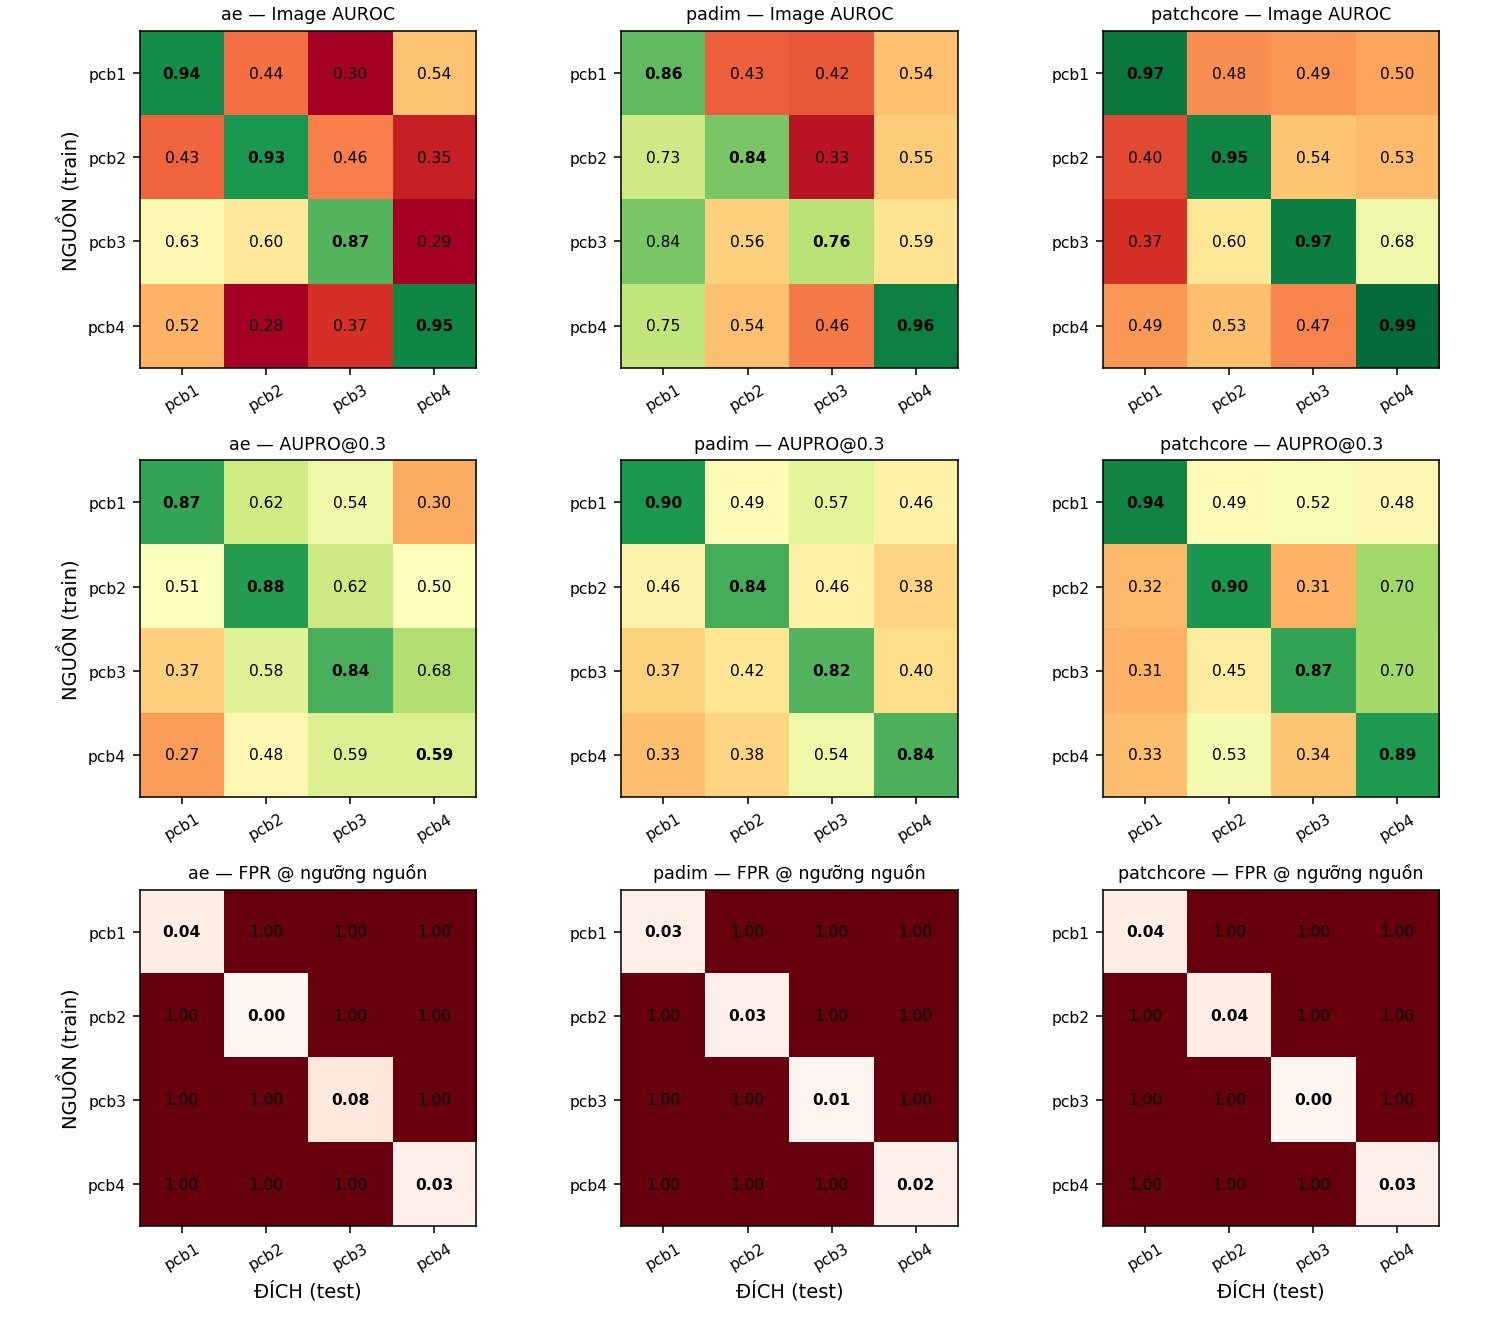
\includegraphics[width=0.8\linewidth]{images/tn/tn3_ma_tran_visa.jpg}
  \caption[Ma trận I-AUROC nguồn và đích trên VisA]{Ma trận image-AUROC nguồn và đích trên VisA pcb1--pcb4 cho ba
    phương pháp (hàng là nguồn, cột là đích)}
  \label{fig:tn3-visa}
\end{figure}

\begin{figure}[htbp]
  \centering
  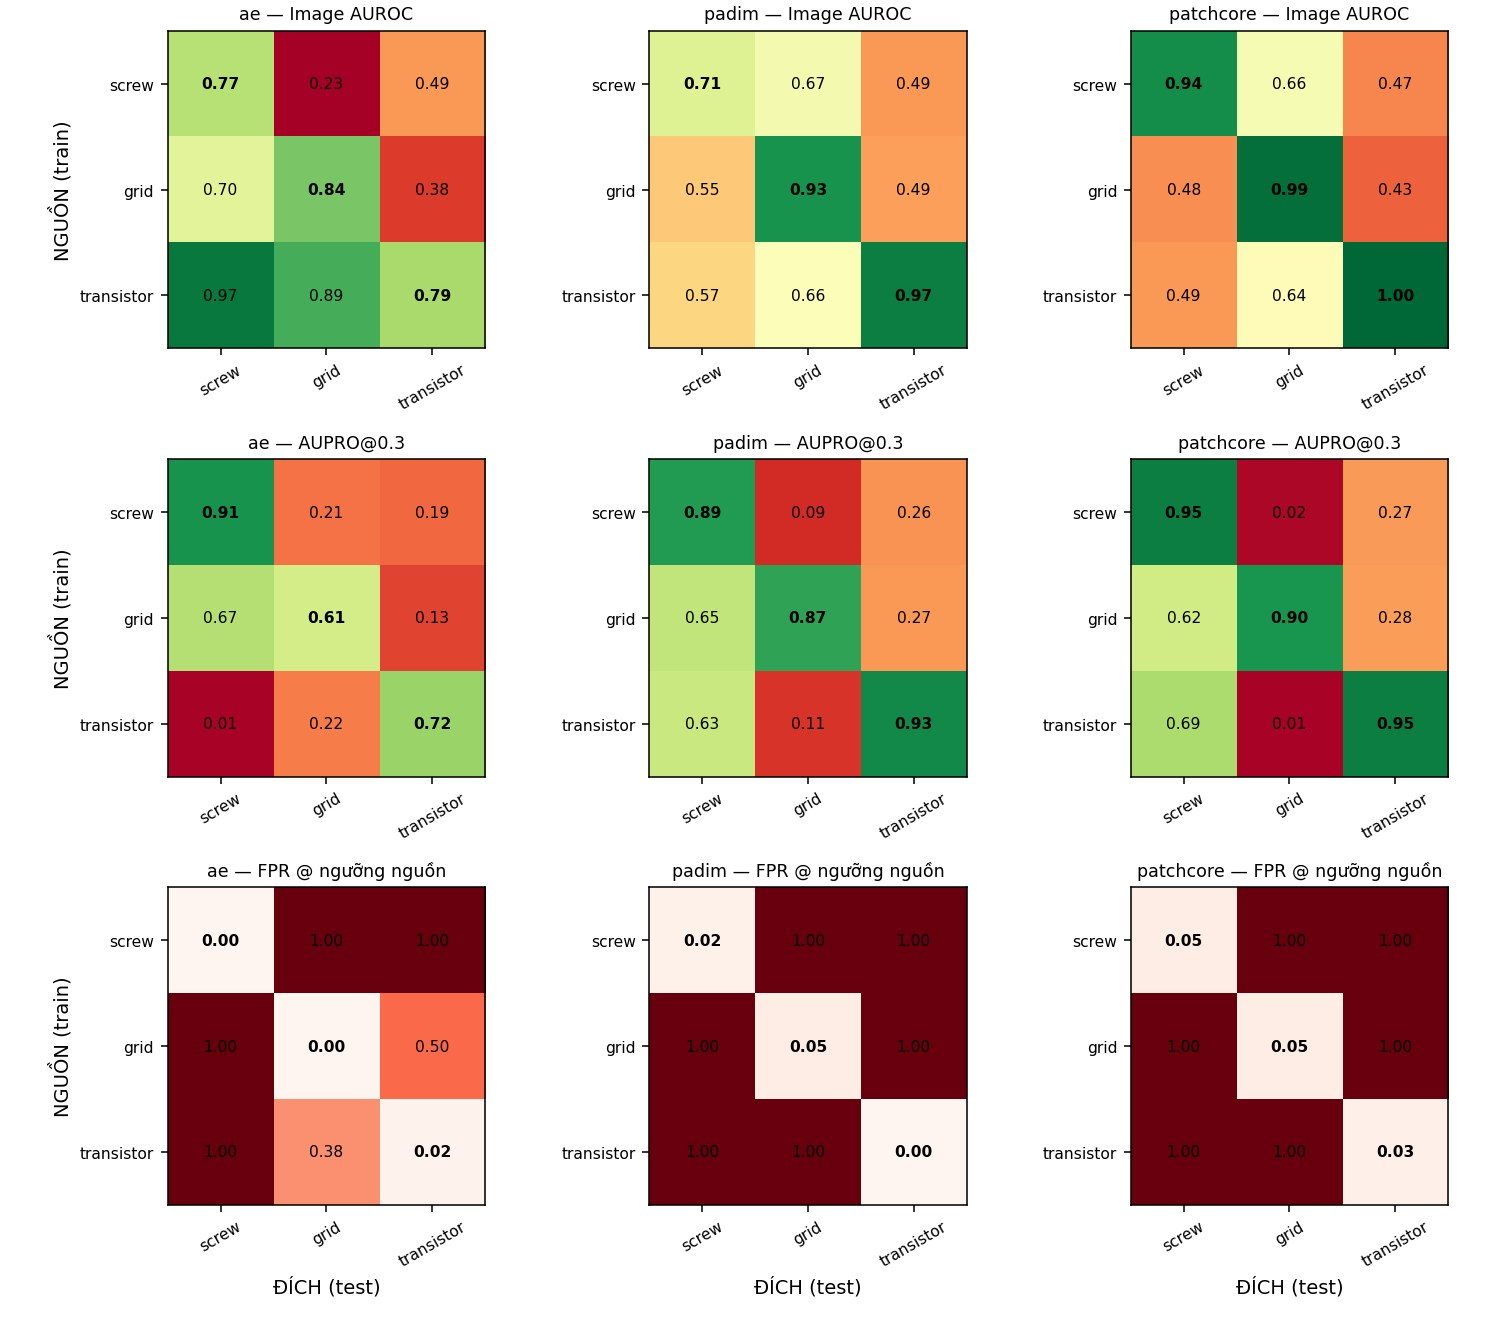
\includegraphics[width=0.8\linewidth]{images/tn/tn3_ma_tran_mvtec.jpg}
  \caption{Ma trận image-AUROC nguồn và đích trên grid, screw, transistor}
  \label{fig:tn3-mvtec}
\end{figure}

\begin{table}[htbp]
  \centering
  \caption{Image-AUROC trung bình trên và ngoài đường chéo của ma trận nguồn và đích}
  \label{tab:tn3}
  \begin{tabular}{@{}llccc@{}}
    \toprule
    Bộ dữ liệu & Vị trí & Autoencoder & PaDiM & PatchCore \\
    \midrule
    VisA     & Đường chéo       & 0,925 & 0,857 & 0,972 \\
             & Ngoài đường chéo & 0,434 & 0,560 & 0,505 \\
    \midrule
    MVTec AD & Đường chéo       & 0,796 & 0,870 & 0,977 \\
             & Ngoài đường chéo & 0,610 & 0,570 & 0,527 \\
    \bottomrule
  \end{tabular}
\end{table}

Ngoài đường chéo, cả ba phương pháp rơi về khoảng 0,43 đến 0,61, tương đương đoán ngẫu nhiên (Bảng~\ref{tab:tn3},
Hình~\ref{fig:tn3-visa} và~\ref{fig:tn3-mvtec}). Tại ngưỡng lấy từ nguồn, mọi cặp ngoài đường chéo có FPR và TPR đều
bằng 100\%: mô hình coi toàn bộ sản phẩm mới là bất thường. Đây là hành vi đúng của một bộ phát hiện bất thường, nhưng
cũng có nghĩa là không dùng lại được mô hình. Sự ``gần'' về loại sản phẩm không giúp gì: pcb1 và pcb2 là hai mặt của
cùng một bảng mạch, nhưng pcb1 sang pcb2 chỉ đạt 0,43--0,48. Với các phương pháp dựa trên đặc trưng cục bộ, ``gần''
phải là gần về bố cục điểm ảnh và kết cấu. Một vài cặp có kết quả cao bất thường, như PaDiM từ pcb3 sang pcb1 (0,837)
và từ pcb2 sang pcb1 (0,733), nhưng không đối xứng, nên nhiều khả năng là trùng hợp về độ tương phản.

Autoencoder có giá trị ngoài đường chéo cao nhất trên MVTec AD (0,610), có vẻ khớp với dự đoán ``linh hoạt hơn''. Nhưng
con số này bị kéo lên bởi một ô duy nhất: Autoencoder từ transistor sang screw đạt 0,975. Đây không phải khả năng tổng
quát thật mà là lối tắt độ sáng ở Mục~\ref{sec:tn2b}: ảnh screw lỗi sáng hơn ảnh screw tốt, và một Autoencoder học trên
transistor dựng kém vùng nền sáng. Trên VisA, nơi không có lối tắt này, Autoencoder lại kém nhất (0,434).

\begin{table}[htbp]
  \centering
  \caption{Image-AUROC khi thích nghi từ nguồn pcb1 sang các loại đích}
  \label{tab:tn3-thich-nghi}
  \small
  \begin{tabular}{@{}llccccc@{}}
    \toprule
    & & \multicolumn{2}{c}{Chỉ ảnh đích} & \multicolumn{2}{c}{Nguồn và ảnh đích} & \\
    \cmidrule(lr){3-4}\cmidrule(lr){5-6}
    Đích & Phương pháp & 4 ảnh & 16 ảnh & 4 ảnh & 16 ảnh & Đích đầy đủ \\
    \midrule
    pcb2 & PatchCore   & 0,88  & 0,86 & 0,91 & 0,92 & 0,96 \\
    pcb3 & PatchCore   & 0,84  & 0,87 & 0,83 & 0,90 & 0,97 \\
    pcb4 & PatchCore   & 0,98  & 0,97 & 0,97 & 0,97 & 0,99 \\
    \midrule
    pcb2 & PaDiM       & 0,66  & 0,79 & 0,55 & 0,65 & -- \\
    pcb3 & PaDiM       & 0,53  & 0,70 & 0,47 & 0,62 & -- \\
    pcb4 & PaDiM       & 0,77  & 0,92 & 0,63 & 0,84 & -- \\
    \midrule
    pcb2 & Autoencoder & 0,73  & 0,69 & 0,63 & 0,79 & -- \\
    pcb3 & Autoencoder & 0,54  & 0,66 & 0,51 & 0,66 & -- \\
    pcb4 & Autoencoder & 0,59  & 0,75 & 0,60 & 0,77 & -- \\
    \bottomrule
  \end{tabular}
\end{table}

\begin{figure}[htbp]
  \centering
  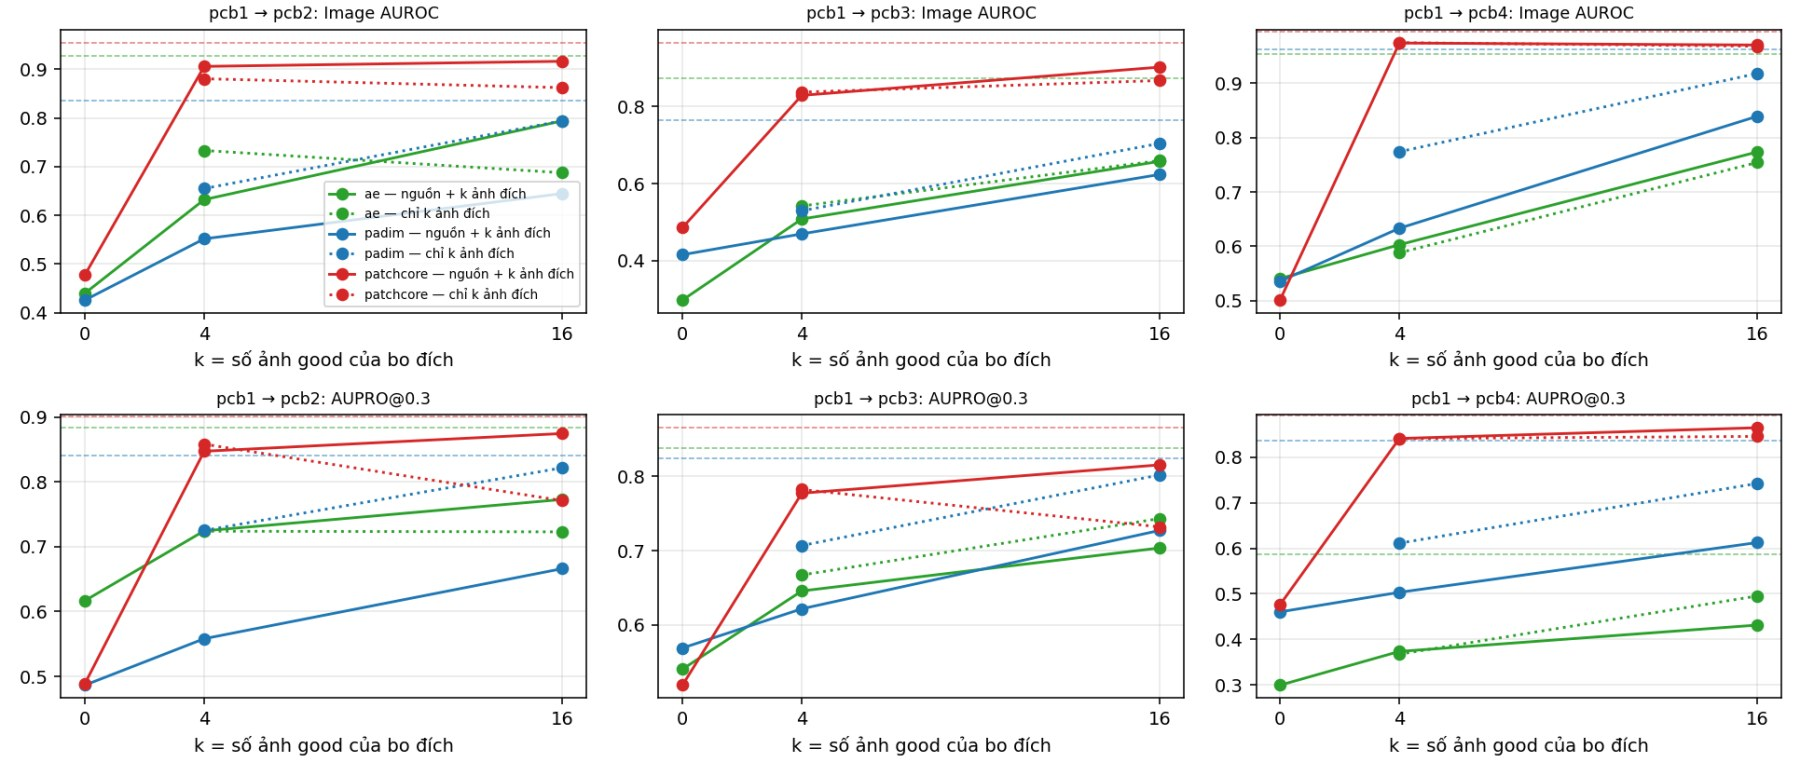
\includegraphics[width=\linewidth]{images/tn/tn3_thich_nghi.jpg}
  \caption[I-AUROC khi thích nghi từ pcb1 sang loại khác]{Image-AUROC khi thích nghi từ pcb1 sang pcb2, pcb3, pcb4 với
    4 và 16 ảnh đích: chỉ ảnh đích so với nguồn cộng ảnh đích}
  \label{fig:tn3-thich-nghi}
\end{figure}

Khả năng thích nghi khác nhau rõ rệt (Bảng~\ref{tab:tn3-thich-nghi}, Hình~\ref{fig:tn3-thich-nghi}). PatchCore thích
nghi nhanh nhất: chỉ 4 ảnh đích đã đưa image-AUROC từ khoảng 0,5 lên 0,84--0,98, cách mô hình xây dựng đầy đủ trên
loại đích 1 đến 13 điểm. Giữ lại bộ nhớ của nguồn không gây hại, vì patch nguồn chỉ là láng giềng thừa, và còn giúp
nhẹ với pcb2, pcb3 khi có 16 ảnh. PaDiM bị hại khi trộn nguồn: dùng cả nguồn thấp hơn chỉ dùng ảnh đích ở mọi ô, ví dụ
pcb4 với 16 ảnh là 0,84 so với 0,92, vì phân phối theo vị trí phải trộn hai bố cục khác nhau. Autoencoder nằm giữa và
không hưởng lợi rõ từ nguồn. Khi đặt lại ngưỡng bằng ảnh tốt của loại đích, FPR quay về 0--5\%.

Không phương pháp nào tổng quát được sang loại sản phẩm khác, kể cả loại ``gần'' nhau. Khi đổi sản phẩm, bắt buộc phải
đặt lại ngưỡng; nếu dùng PatchCore thì chỉ cần thêm vài ảnh của sản phẩm mới vào bộ nhớ. Một kết quả cao bất thường
như Autoencoder từ transistor sang screw cần được nghi ngờ và kiểm tra lối tắt trong dữ liệu trước khi kết luận.

\subsection{Thí nghiệm 4: thay đổi điều kiện chụp}
\label{sec:tn4}

Sau khi triển khai, đèn có thể yếu đi, camera mất nét, cảm biến nhiễu hơn hoặc sản phẩm bị lệch vị trí, trong khi mô
hình không được huấn luyện lại và ngưỡng đã chốt. Nhóm đặt ba giả thuyết từ cơ chế: H1, PatchCore nhạy với ánh sáng
vì so khớp tuyệt đối với patch đã ghi nhớ; H2, PaDiM nhạy với nhiễu vì nhiễu đẩy đặc trưng ra ngoài phân phối Gauss hẹp
tại từng vị trí; H3, Autoencoder nhạy với dịch và xoay vì lớp kết nối đầy đủ ở cổ chai gắn với vị trí tuyệt đối. Tiêu
chí chính là FPR trên ảnh tốt tại ngưỡng cố định và mức thay đổi AUPRO, vì AUROC không phụ thuộc ngưỡng.

Có hai loại thay đổi. Thay đổi tạo nhân tạo áp lên tập test của grid, screw, transistor sau khi mô hình và ngưỡng đã
được xây dựng trên ảnh gốc: làm mờ ($\sigma$ = 1, 2, 3), đổi độ sáng (nhân 0,6 đến 1,4), thêm nhiễu Gauss ($\sigma$ =
5 đến 20), xoay (tới 20°, riêng transistor tới 5°) và dịch (tới 32 điểm ảnh, riêng transistor tới 8 điểm ảnh). Xoay và
dịch được thực hiện ở độ phân giải gốc; vùng biên bị đệm (32 điểm ảnh) được loại khỏi đánh giá, cùng những ảnh có lỗi
bị đẩy ra ngoài khung. Thay đổi thật lấy từ tập \texttt{test\_public} của MVTec AD 2, chụp ở các điều kiện bình
thường, quá sáng, quá tối và bốn mức dịch ánh sáng.

\begin{table}[htbp]
  \centering
  \caption[Thay đổi AUPRO và FPR tại ngưỡng cố định ở mức thay đổi mạnh nhất]{Thay đổi AUPRO và FPR tại ngưỡng cố định
    ở mức thay đổi mạnh nhất (thứ tự trong mỗi ô: Autoencoder / PaDiM / PatchCore; FPR gốc của cả ba khoảng 0--5\%)}
  \label{tab:tn4}
  \small
  \begin{tabular}{@{}llcc@{}}
    \toprule
    Thay đổi & Loại & Thay đổi AUPRO & FPR \\
    \midrule
    Làm mờ $\sigma = 3$ & grid       & $-0{,}03$ / $-0{,}25$ / $-0{,}74$ & 0\% / 5\% / 100\% \\
                        & screw      & $-0{,}01$ / $-0{,}14$ / $-0{,}17$ & 0\% / 88\% / 100\% \\
                        & transistor & $-0{,}07$ / $-0{,}24$ / $-0{,}29$ & 0\% / 13\% / 100\% \\
    \midrule
    Độ sáng $\times0{,}6$ & grid       & $-0{,}10$ / $+0{,}01$ / $-0{,}02$ & 0\% / 0\% / 24\% \\
                          & screw      & $-0{,}77$ / $-0{,}01$ / $-0{,}04$ & 100\% / 2\% / 46\% \\
                          & transistor & $-0{,}47$ / $0$ / $0$             & 0\% / 0\% / 10\% \\
    \midrule
    Nhiễu $\sigma = 20$ & grid       & $0$ / $-0{,}46$ / $-0{,}48$       & 0\% / 100\% / 100\% \\
                        & screw      & $0$ / $-0{,}09$ / $-0{,}14$       & 0\% / 100\% / 100\% \\
                        & transistor & $-0{,}05$ / $-0{,}36$ / $-0{,}17$ & 3\% / 100\% / 100\% \\
    \midrule
    Xoay 20° (transistor 5°) & grid       & $+0{,}18$ / $+0{,}06$ / $+0{,}05$ & 0\% / 0\% / 38\% \\
                             & screw      & $-0{,}07$ / $-0{,}02$ / $0$       & 51\% / 10\% / 12\% \\
                             & transistor & $-0{,}29$ / $-0{,}17$ / $0$       & 5\% / 92\% / 18\% \\
    \midrule
    Dịch 32 điểm ảnh (transistor 8) & grid       & $+0{,}18$ / $+0{,}03$ / $-0{,}02$ & 0\% / 0\% / 100\% \\
                                    & screw      & $-0{,}20$ / $-0{,}11$ / $-0{,}08$ & 100\% / 95\% / 100\% \\
                                    & transistor & $-0{,}28$ / $-0{,}20$ / $0$       & 15\% / 67\% / 5\% \\
    \bottomrule
  \end{tabular}
\end{table}

\begin{figure}[htbp]
  \centering
  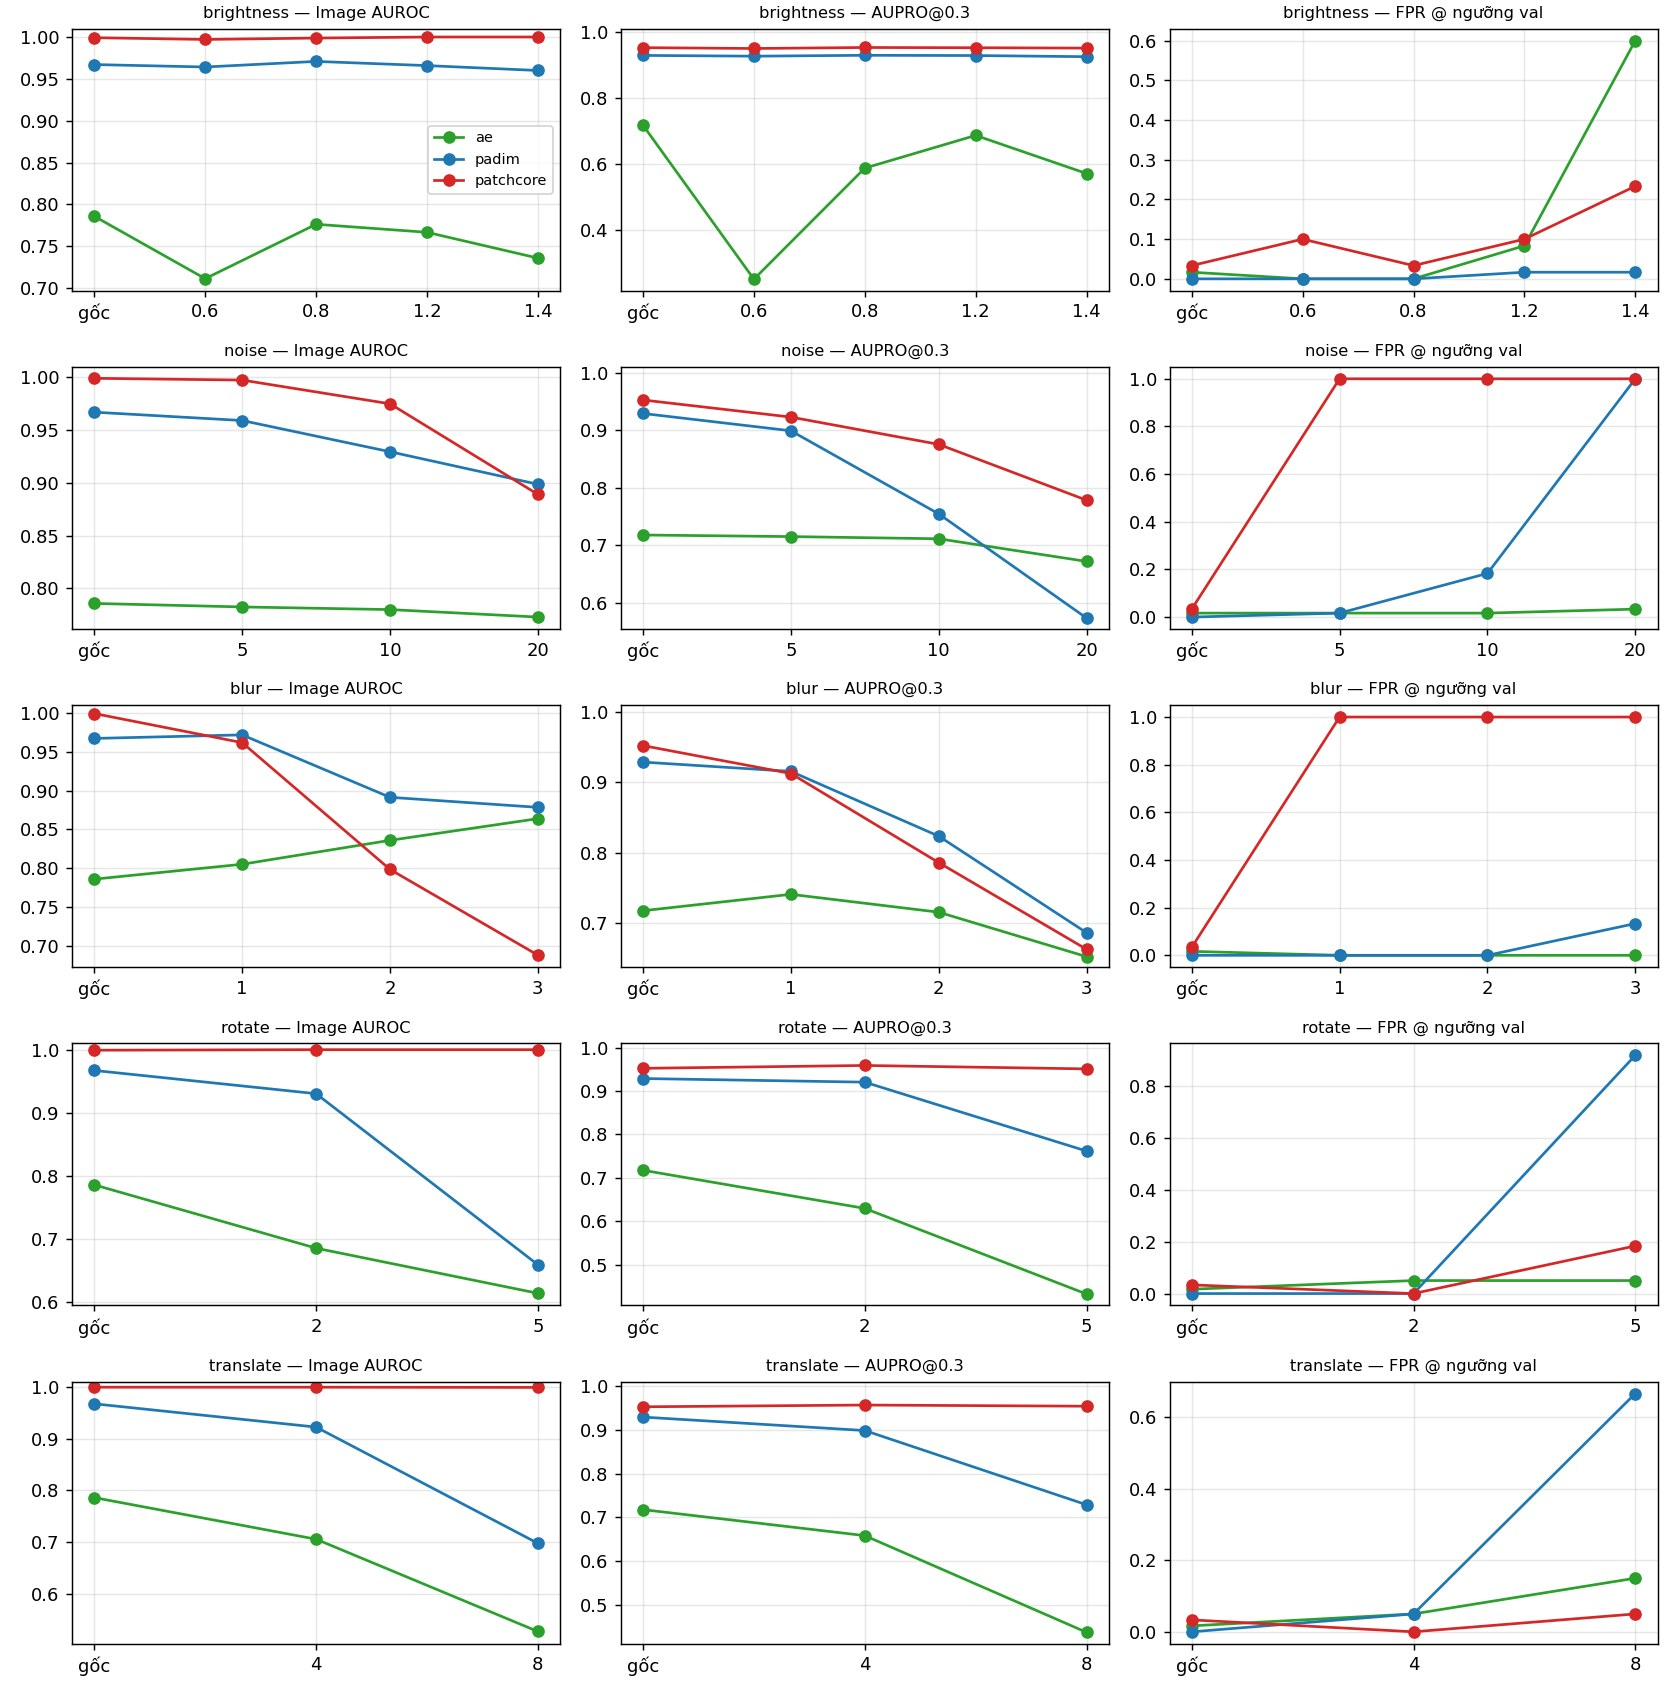
\includegraphics[width=0.8\linewidth]{images/tn/tn4_shift_transistor.jpg}
  \caption{I-AUROC, AUPRO và FPR theo cường độ từng loại thay đổi trên transistor}
  \label{fig:tn4-transistor}
\end{figure}

\begin{figure}[htbp]
  \centering
  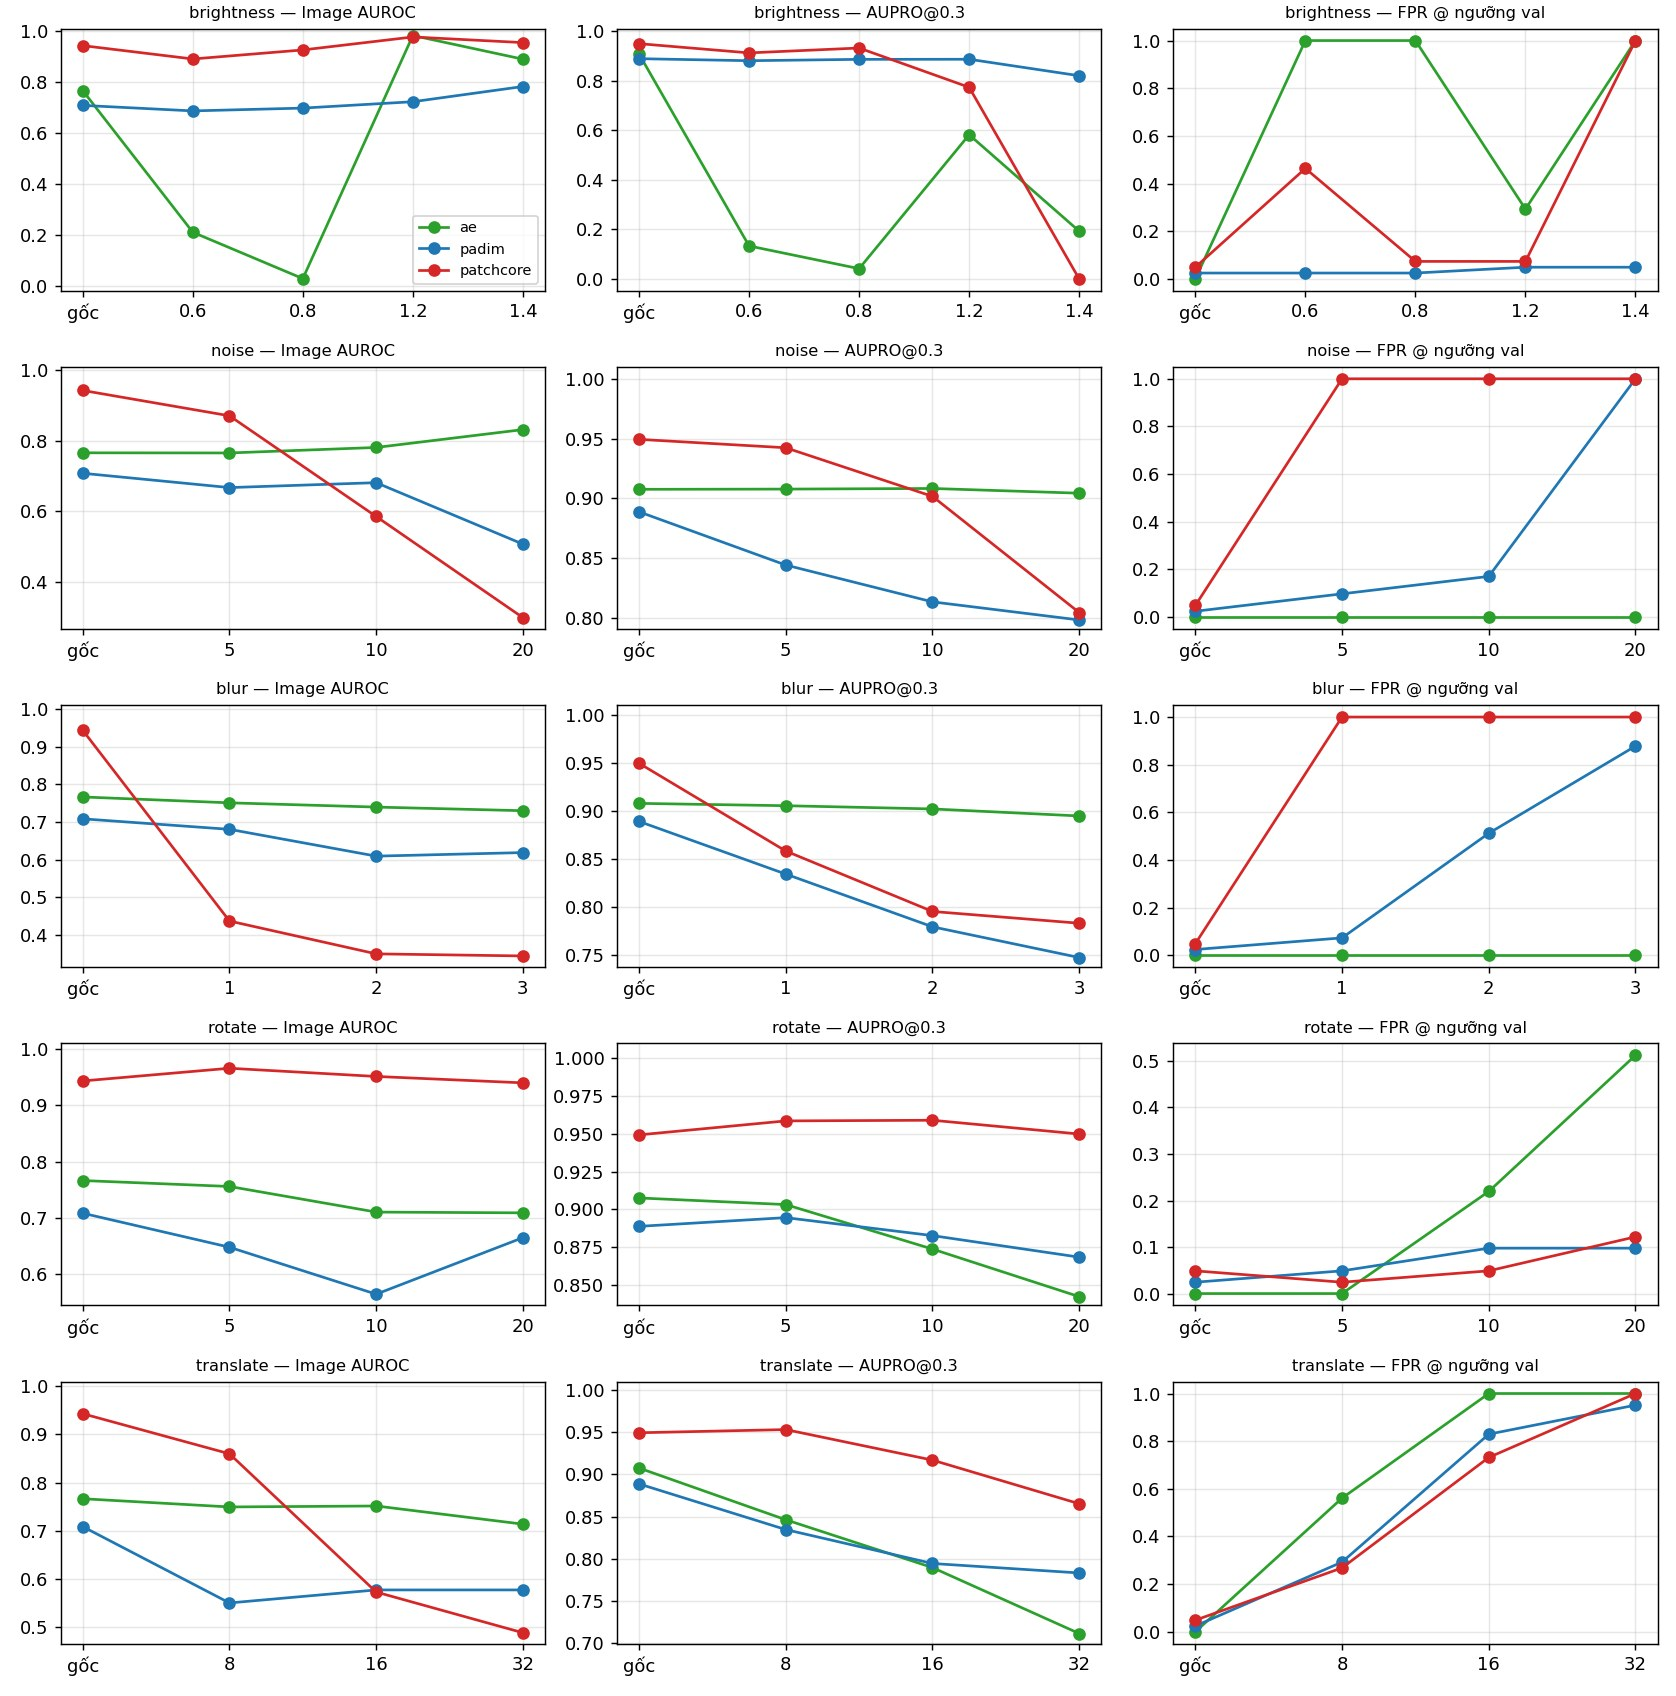
\includegraphics[width=0.8\linewidth]{images/tn/tn4_shift_screw.jpg}
  \caption{I-AUROC, AUPRO và FPR theo cường độ từng loại thay đổi trên screw}
  \label{fig:tn4-screw}
\end{figure}

Bảng~\ref{tab:tn4} và Hình~\ref{fig:tn4-transistor},~\ref{fig:tn4-screw} cho kết quả ở mức thay đổi mạnh nhất. Dòng
dịch trên screw và grid có thể còn bị ảnh hưởng bởi vùng biên nên không dùng để kết luận. Giả thuyết H1 bị bác bỏ với
ánh sáng tạo nhân tạo: giảm độ sáng xuống 0,6 lần hầu như không đổi AUPRO của PatchCore (từ $-0{,}04$ đến 0), vì đặc
trưng từ backbone ImageNet khá bất biến với thay đổi độ sáng toàn ảnh; dù vậy FPR vẫn tăng (46\% trên screw), và với
ánh sáng thật thì giả thuyết đúng một phần. Giả thuyết H2 đúng nhưng không riêng PaDiM: nhiễu $\sigma = 20$ đẩy FPR của
PaDiM lên 100\% ở cả ba loại, và PatchCore bị nặng tương đương, vì hai phương pháp dùng chung backbone nên cùng nhạy
với nhiễu tần số cao. Giả thuyết H3 đúng trên transistor: xoay 5° làm AUPRO của Autoencoder giảm 0,29, dịch 8 điểm ảnh
giảm 0,28, trong khi PatchCore không đổi. PaDiM cũng rất nhạy (FPR 92\% khi xoay 5°, 67\% khi dịch 8 điểm ảnh), đúng
với cơ chế phân phối theo vị trí dù giả thuyết ban đầu không nêu.

Ba phát hiện nằm ngoài giả thuyết. Thứ nhất, Autoencoder sụp đổ với độ sáng: chỉ giảm độ sáng còn 0,8 lần trên screw đã
làm image-AUROC giảm 0,74 và FPR thành 100\%, vì mạng tối ưu MSE theo cường độ điểm ảnh nên mọi thay đổi cường độ đều
thành sai số tái tạo; đây cũng là cơ chế của lối tắt độ sáng ở Mục~\ref{sec:tn2b}. Thứ hai, PatchCore rất nhạy với làm
mờ: chỉ $\sigma = 1$ trên screw đã làm image-AUROC giảm 0,51 và FPR thành 100\%, còn trên grid AUPRO giảm 0,74, vì
PatchCore dựa vào chi tiết kết cấu tần số cao, đúng thứ mà làm mờ xóa đi; ngược lại, Autoencoder gần như không bị ảnh
hưởng bởi làm mờ và nhiễu vì bản thân nó đã dựng ra ảnh mờ. Thứ ba, AUROC che giấu thất bại: trên transistor, nhiễu
$\sigma = 5$ làm image-AUROC của PatchCore gần như không đổi nhưng FPR tăng từ 3\% lên 100\%. Mô hình vẫn xếp hạng đúng
nhưng mọi điểm bị đẩy vượt ngưỡng; trên dây chuyền, mọi sản phẩm sẽ bị loại.

Hai mức hỏng không đi cùng nhau. Nhiễu và làm mờ chủ yếu gây báo nhầm hàng loạt, với bản đồ sáng đều trên toàn ảnh.
Độ sáng với Autoencoder và xoay, dịch với PaDiM gây bản đồ sai chỗ: AUPRO giảm mạnh vì vùng sáng nằm ở biên vật thể
thay vì ở vùng lỗi.

\begin{table}[htbp]
  \centering
  \caption[Kết quả trên vial theo điều kiện chụp]{Kết quả trên vial theo điều kiện chụp (thứ tự trong mỗi ô:
    Autoencoder / PaDiM / PatchCore)}
  \label{tab:tn4-vial}
  \small
  \begin{tabular}{@{}lcc@{}}
    \toprule
    Điều kiện & Image-AUROC & AUPRO \\
    \midrule
    Bình thường & 0,72 / 0,787 / 0,907 & 0,841 / 0,898 / 0,887 \\
    Quá sáng    & 0,547 / 0,413 / 0,920 & 0,755 / 0,555 / 0,793 \\
    Quá tối     & 0,653 / 0,507 / 0,667 & 0,657 / 0,318 / 0,542 \\
    Dịch ánh sáng 1--4 & 0,68--0,75 / 0,68--0,80 / 0,907--0,92 & -- \\
    \bottomrule
  \end{tabular}
\end{table}

\begin{figure}[htbp]
  \centering
  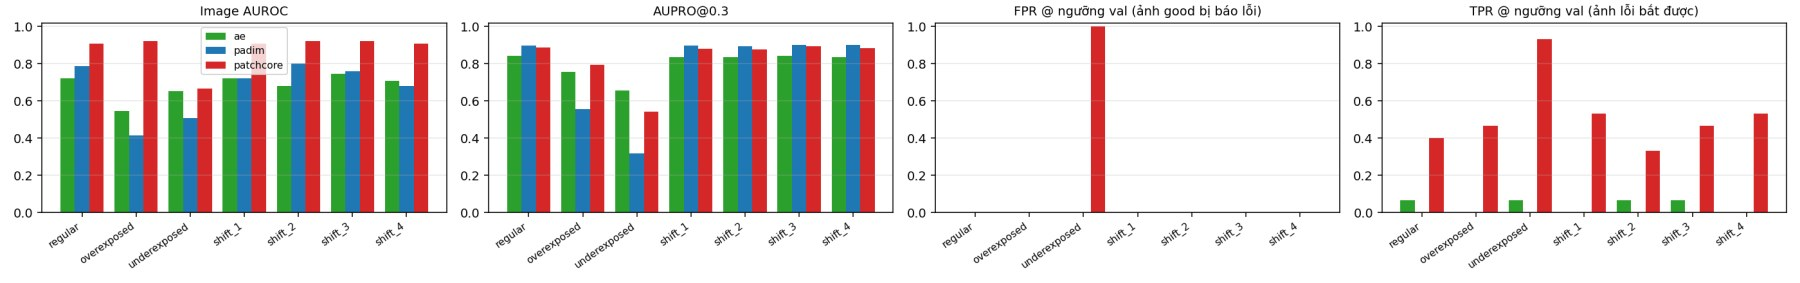
\includegraphics[width=\linewidth]{images/tn/tn4_vial_dieu_kien.jpg}
  \caption{I-AUROC và AUPRO của ba phương pháp trên vial theo từng điều kiện chụp}
  \label{fig:tn4-vial}
\end{figure}

\begin{figure}[htbp]
  \centering
  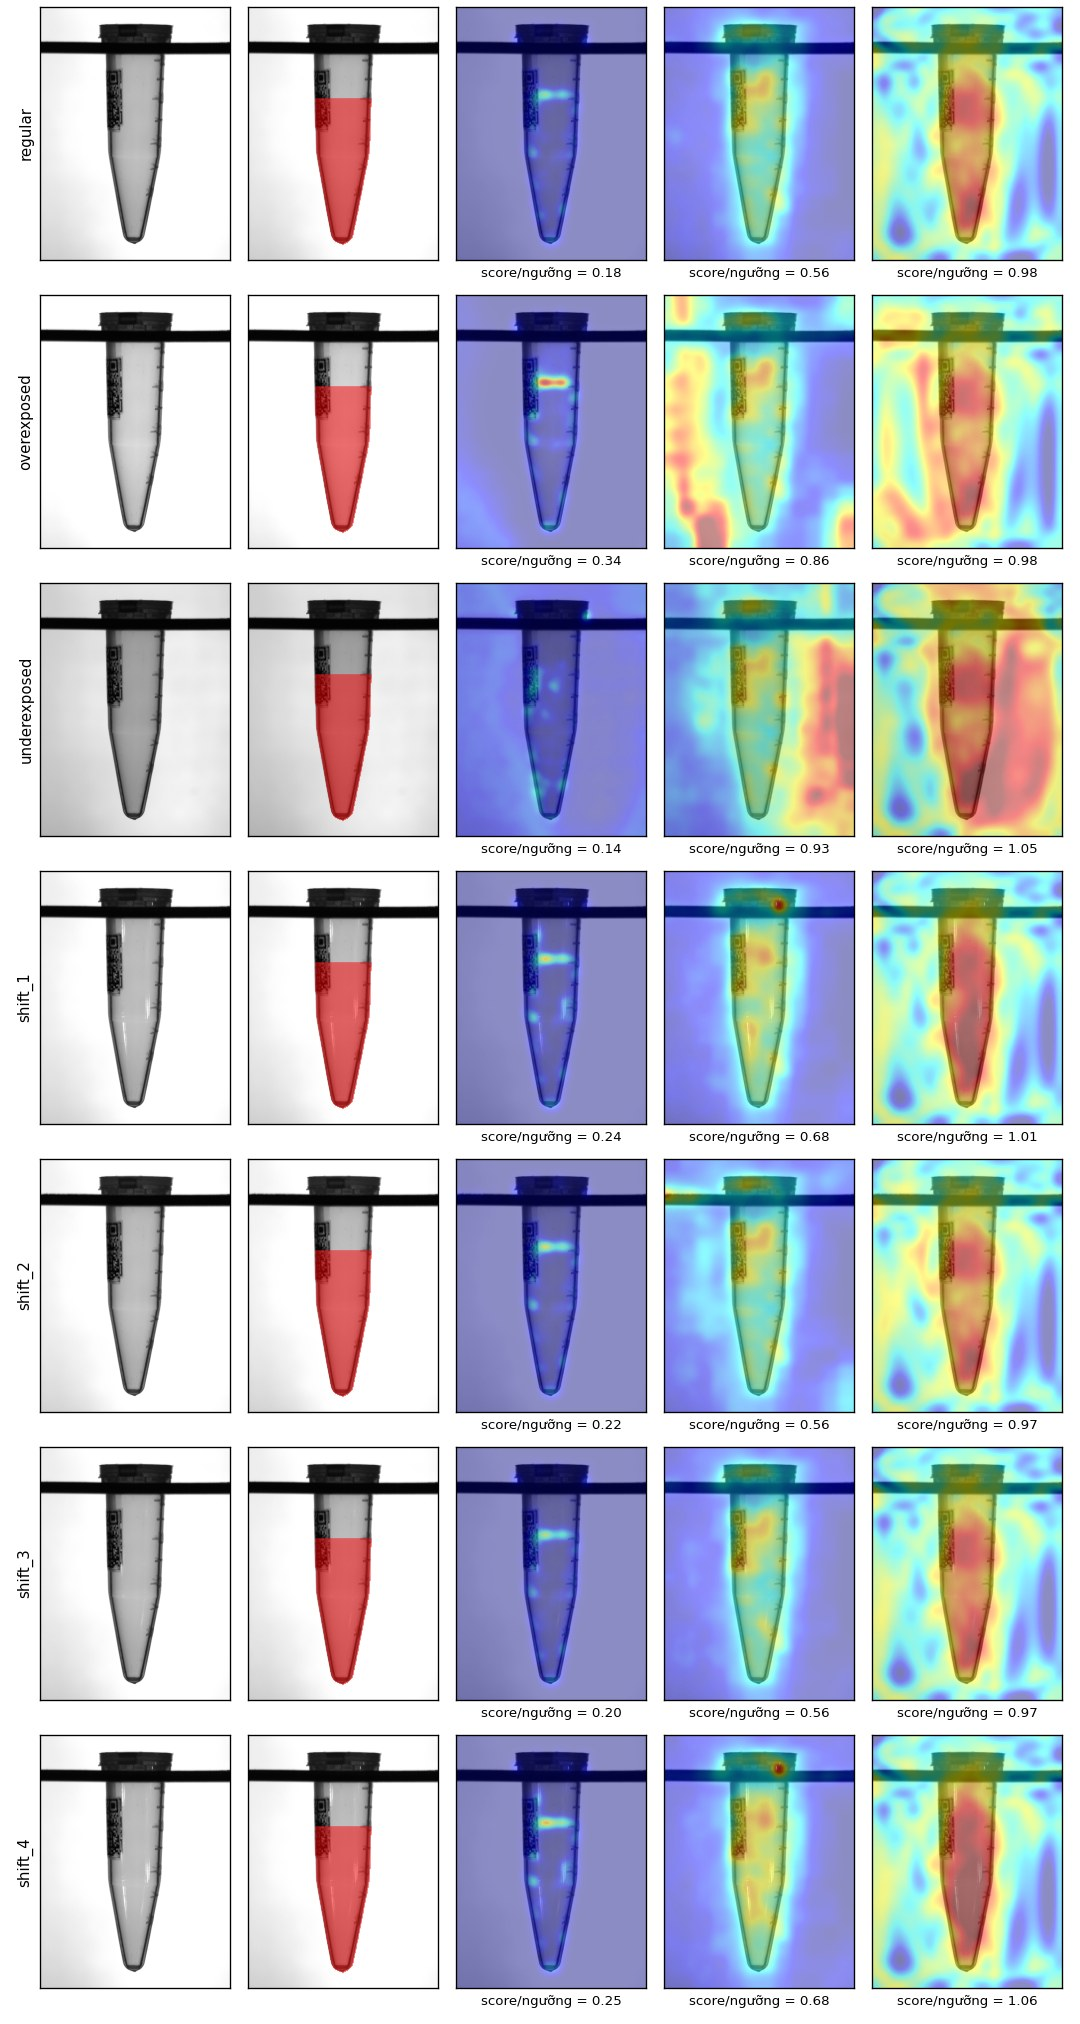
\includegraphics[width=0.45\linewidth]{images/tn/tn4_vial_heatmap.jpg}
  \caption[Cùng một cảnh vial ở ba điều kiện chụp]{Cùng một cảnh vial ở điều kiện bình thường, quá sáng và quá tối,
    cùng bản đồ bất thường của ba phương pháp}
  \label{fig:tn4-vial-heatmap}
\end{figure}

\begin{figure}[htbp]
  \centering
  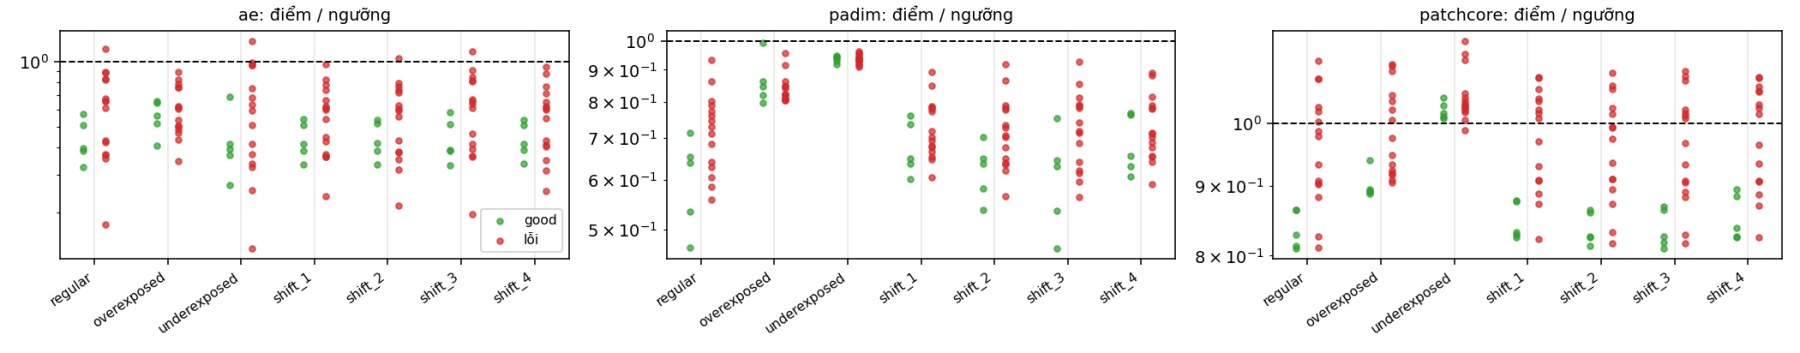
\includegraphics[width=\linewidth]{images/tn/tn4_vial_phan_phoi.jpg}
  \caption[Phân phối điểm trên vial theo điều kiện ánh sáng]{Phân phối điểm bất thường của ảnh tốt và ảnh lỗi trên vial
    theo điều kiện ánh sáng, so với ngưỡng cố định}
  \label{fig:tn4-vial-phan-phoi}
\end{figure}

Với ánh sáng thật trên vial (Bảng~\ref{tab:tn4-vial}, Hình~\ref{fig:tn4-vial} đến~\ref{fig:tn4-vial-phan-phoi}), PaDiM
sụp đổ: image-AUROC 0,413 khi quá sáng và 0,507 khi quá tối, tức bằng hoặc dưới mức ngẫu nhiên, còn AUPRO giảm từ
0,898 xuống 0,318. Khác với ánh sáng tạo nhân tạo vốn nhân đều cả ảnh, ánh sáng thật thay đổi phản xạ và độ bão hòa
cục bộ trên thủy tinh, nên làm lệch phân phối tại những vị trí cụ thể. PatchCore bền với ảnh quá sáng và các mức dịch
ánh sáng (0,907--0,92) nhưng yếu khi ảnh quá tối, với image-AUROC 0,667 và FPR 100\% tại ngưỡng cố định, khớp với
Bảng~\ref{tab:vial-cond}. Đây là phần đúng của H1: PatchCore bền với thay đổi độ sáng tuyến tính nhưng không bền khi
thiếu sáng làm mất chi tiết kết cấu, tương tự làm mờ. Autoencoder giảm vừa phải và đều, và giữ AUPRO tốt nhất khi ảnh
quá tối (0,657).

\begin{figure}[htbp]
  \centering
  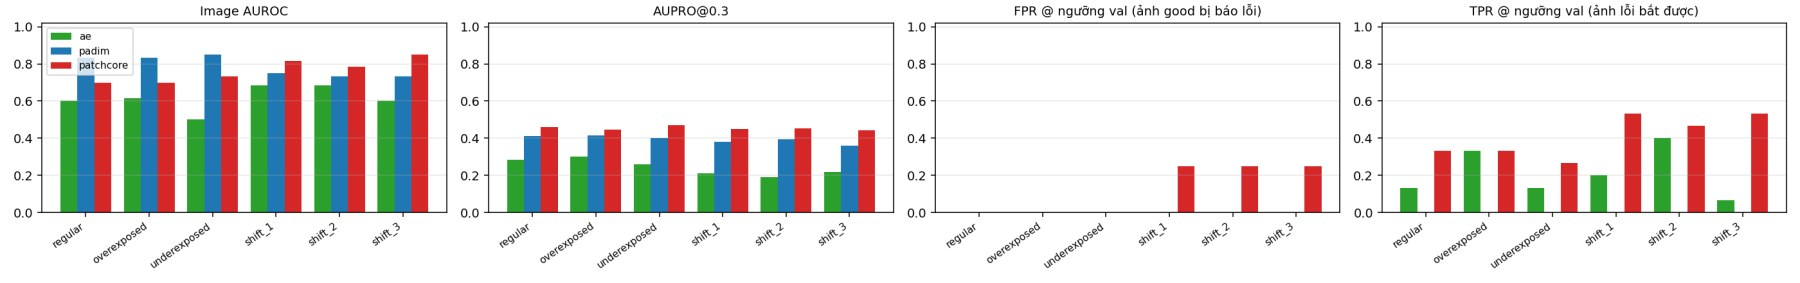
\includegraphics[width=\linewidth]{images/tn/tn4_sheet_metal.jpg}
  \caption{I-AUROC và AUPRO trên sheet\_metal theo từng điều kiện chụp}
  \label{fig:tn4-sheet}
\end{figure}

Sheet\_metal cho thấy một kiểu thất bại khác (Hình~\ref{fig:tn4-sheet}). Image-AUROC của PaDiM và PatchCore khá ổn
định qua các điều kiện (0,70--0,85), của Autoencoder là 0,50--0,68, nhưng khả năng định vị rất kém ở mọi điều kiện:
AUPRO khoảng 0,39 với PaDiM, 0,45 với PatchCore và 0,25 với Autoencoder. Ảnh sheet\_metal rất dài với lỗi nhỏ và mảnh,
nên vấn đề chính không phải thay đổi điều kiện chụp mà là đặc trưng quá thô so với kích thước lỗi. Vial hỏng theo điều
kiện, tức ánh sáng thay đổi thì báo nhầm hàng loạt; sheet\_metal hỏng ở mọi điều kiện, tức bỏ sót lỗi nhỏ và bản đồ
không trùng lỗi. Hai loại cần hai cách khắc phục khác nhau: chuẩn hóa ánh sáng hoặc tăng cường dữ liệu cho vial, cắt
ảnh thành nhiều mảnh hoặc dùng đặc trưng độ phân giải cao cho sheet\_metal.

\begin{table}[htbp]
  \centering
  \caption{Độ nhạy của ba phương pháp với thay đổi điều kiện chụp}
  \label{tab:tn4-tom-tat}
  \small
  \begin{tabular}{@{}l>{\raggedright\arraybackslash}p{3.6cm}>{\raggedright\arraybackslash}p{3.2cm}>{\raggedright\arraybackslash}p{4.6cm}@{}}
    \toprule
    Phương pháp & Nhạy nhất với & Bền với & Giải thích \\
    \midrule
    Autoencoder & Độ sáng; dịch, xoay (transistor) & Làm mờ, nhiễu & MSE trên cường độ điểm ảnh; cổ chai gắn vị trí \\
    PaDiM & Nhiễu; ánh sáng thật; dịch, xoay & Độ sáng tạo nhân tạo & Phân phối Gauss hẹp, theo từng vị trí \\
    PatchCore & Làm mờ, nhiễu, ảnh quá tối & Độ sáng tạo nhân tạo; dịch, xoay (theo AUPRO; FPR vẫn tăng) & Dựa vào chi
      tiết kết cấu; so khớp không theo vị trí \\
    \bottomrule
  \end{tabular}
\end{table}

Không phương pháp nào bền với mọi loại thay đổi (Bảng~\ref{tab:tn4-tom-tat}); lựa chọn nên dựa vào loại biến động hay
gặp nhất ở dây chuyền. Quan trọng hơn, cần theo dõi FPR trên ảnh tốt theo thời gian, vì AUROC có thể không đổi trong
khi hệ thống đã báo lỗi mọi sản phẩm.

\subsection{Thí nghiệm 5: phân tích theo kiểu lỗi và các ca thất bại}
\label{sec:tn5}

Các con số trung bình che giấu kiểu thất bại. Từ cơ chế, nhóm dự đoán Autoencoder thất bại khi tái tạo quá tốt (dựng
lại cả lỗi nên bỏ sót) hoặc quá kém (sai số cao ở vùng chi tiết hay vùng sáng bình thường nên báo nhầm); PaDiM thất bại
khi giả định phân phối Gauss theo vị trí bị vi phạm; PatchCore thất bại khi đặc trưng quá thô so với lỗi, hoặc khi
một patch tốt hiếm gặp không có láng giềng trong bộ nhớ. Bảng~\ref{tab:tn5-screw} và~\ref{tab:tn5-khac} cho
image-AUROC của từng kiểu lỗi, tính trên ảnh lỗi kiểu đó so với toàn bộ ảnh tốt.

\begin{table}[htbp]
  \centering
  \caption{Image-AUROC theo từng kiểu lỗi của screw}
  \label{tab:tn5-screw}
  \begin{tabular}{@{}llccc@{}}
    \toprule
    Nhóm lỗi & Kiểu lỗi & Autoencoder & PaDiM & PatchCore \\
    \midrule
    Lỗi ren     & thread\_side       & 0,643 & 0,631 & 0,917 \\
                & thread\_top        & 0,854 & 0,687 & 0,995 \\
    Lỗi đầu     & scratch\_head      & 0,787 & 0,737 & 0,947 \\
    Biến dạng   & manipulated\_front & 0,841 & 0,772 & 0,928 \\
    Lỗi thân, cổ & scratch\_neck     & 0,806 & 0,778 & 0,987 \\
    \bottomrule
  \end{tabular}
\end{table}

\begin{figure}[htbp]
  \centering
  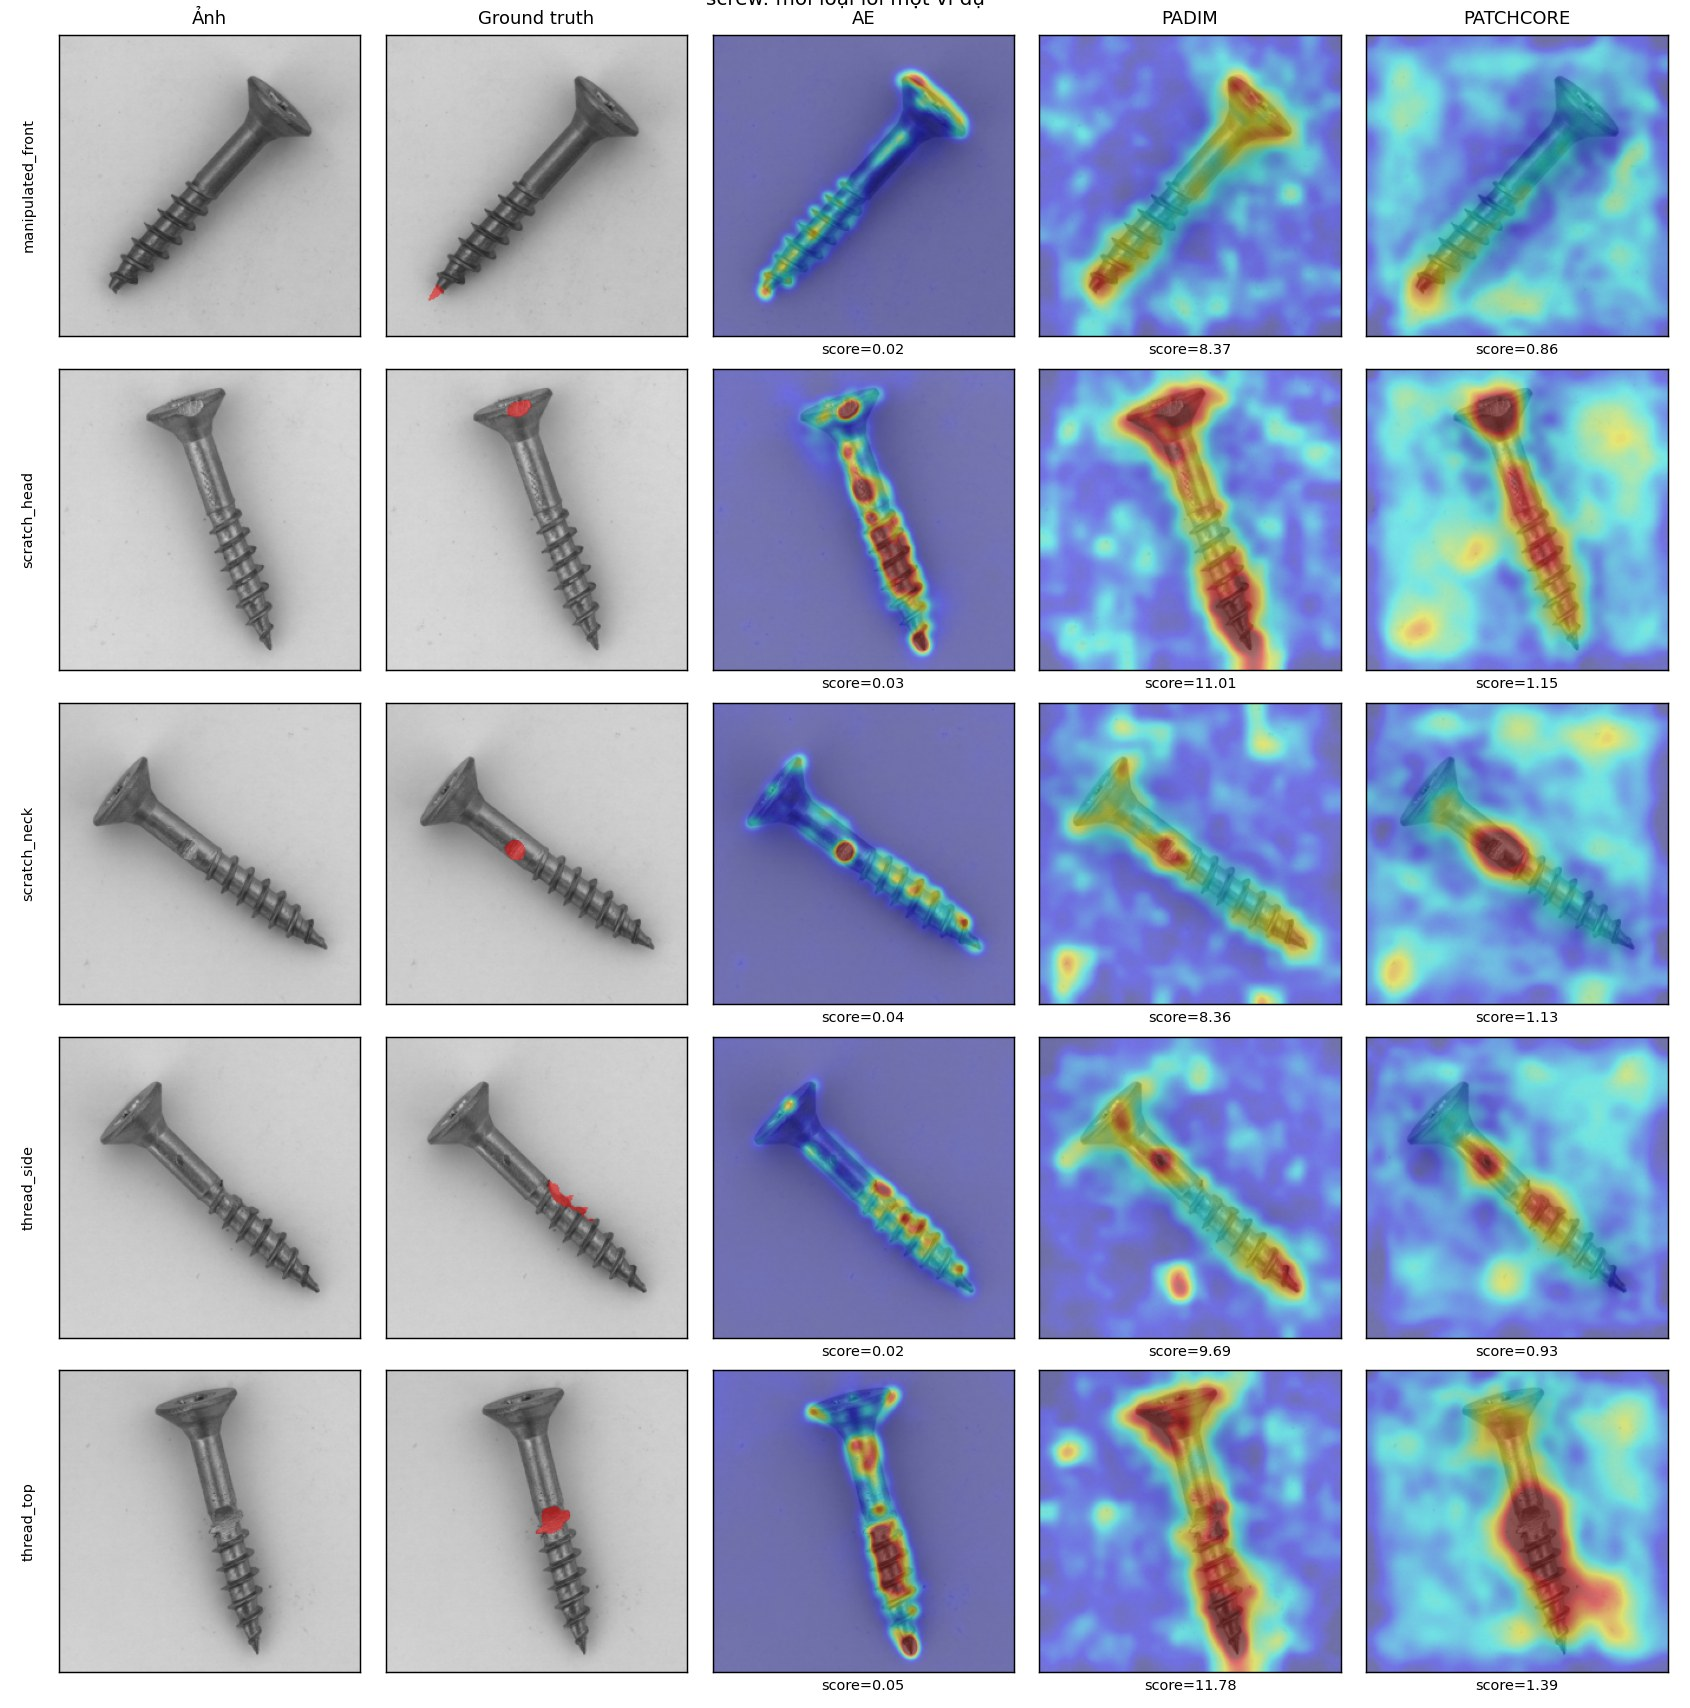
\includegraphics[width=0.8\linewidth]{images/tn/tn5_screw_loai_loi.jpg}
  \caption[Ví dụ từng kiểu lỗi của screw]{Ví dụ từng kiểu lỗi của screw: ảnh gốc, mặt nạ lỗi và bản đồ của
    Autoencoder, PaDiM, PatchCore}
  \label{fig:tn5-screw}
\end{figure}

Lỗi ren bên thân (thread\_side) khó nhất với cả ba (Bảng~\ref{tab:tn5-screw}, Hình~\ref{fig:tn5-screw}). Ren vít là cấu
trúc lặp lại tần số cao, nên một đoạn ren hỏng vẫn trông giống ren ở mức đặc trưng thô. Autoencoder (0,643) dựng ren
thành một dải mờ, nên sai số ở ren tốt và ren hỏng như nhau; đây là kiểu ``tái tạo quá kém ở mọi nơi''. PaDiM (0,631)
thất bại vì ren nằm ở vị trí khác nhau tùy góc xoay, và PaDiM yếu đều ở mọi nhóm lỗi của screw (0,63--0,78), tức thất
bại do giả định căn chỉnh chứ không phải do kiểu lỗi. PatchCore đạt từ 0,917 trở lên ở mọi nhóm, yếu nhất cũng ở
thread\_side, khớp với dự đoán đặc trưng quá thô với lỗi nhỏ lặp lại.

\begin{table}[htbp]
  \centering
  \caption{Image-AUROC theo từng kiểu lỗi của transistor và grid}
  \label{tab:tn5-khac}
  \begin{tabular}{@{}llccc@{}}
    \toprule
    Loại & Kiểu lỗi & Autoencoder & PaDiM & PatchCore \\
    \midrule
    transistor & bent\_lead           & 0,802 & 1,000 & 0,998 \\
               & cut\_lead            & 0,692 & 0,978 & 1,000 \\
               & damaged\_case        & 0,542 & 0,895 & 1,000 \\
               & misplaced            & 0,978 & 1,000 & 0,997 \\
    \midrule
    grid       & bent                 & 0,877 & 0,972 & 1,000 \\
               & broken               & 0,758 & 0,996 & 1,000 \\
               & glue                 & 0,706 & 0,870 & 0,961 \\
               & metal\_contamination & 0,922 & 0,996 & 0,996 \\
               & thread               & 0,866 & 0,827 & 0,987 \\
    \bottomrule
  \end{tabular}
\end{table}

\begin{figure}[htbp]
  \centering
  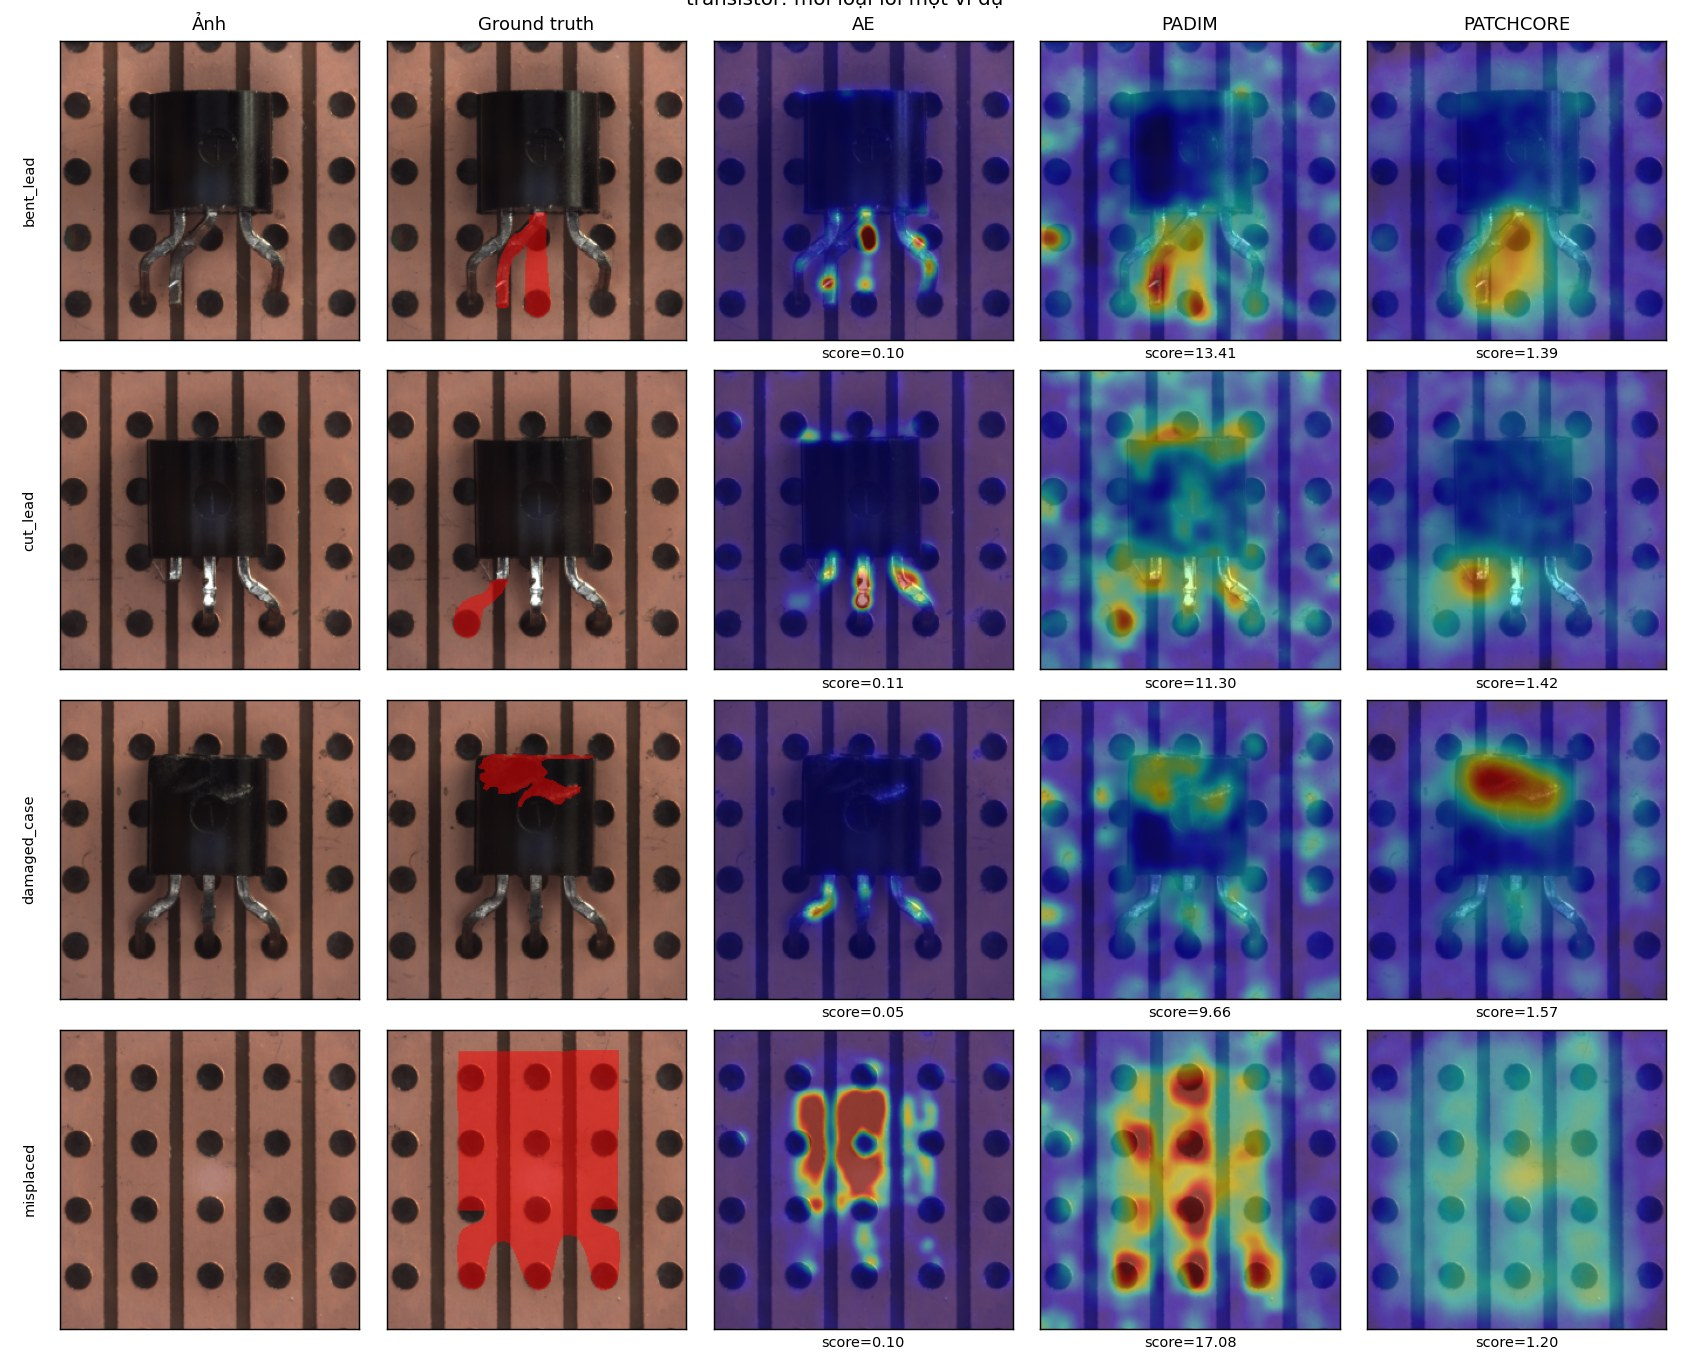
\includegraphics[width=0.8\linewidth]{images/tn/tn5_transistor_loai_loi.jpg}
  \caption{Ví dụ từng kiểu lỗi của transistor với bản đồ của ba phương pháp}
  \label{fig:tn5-transistor}
\end{figure}

Trên transistor (Bảng~\ref{tab:tn5-khac}, Hình~\ref{fig:tn5-transistor}), lỗi misplaced, tức thiếu hoặc lệch cả linh
kiện, là kiểu duy nhất Autoencoder làm tốt (0,978), vì lỗi lớn và thay đổi cấu trúc toàn cục. Lỗi damaged\_case, vết
xước trên vỏ đen, gần như vô hình với Autoencoder (0,542): vết xước tối trên nền tối cho sai số MSE rất nhỏ, đúng kiểu
``tái tạo quá tốt''.

\begin{figure}[htbp]
  \centering
  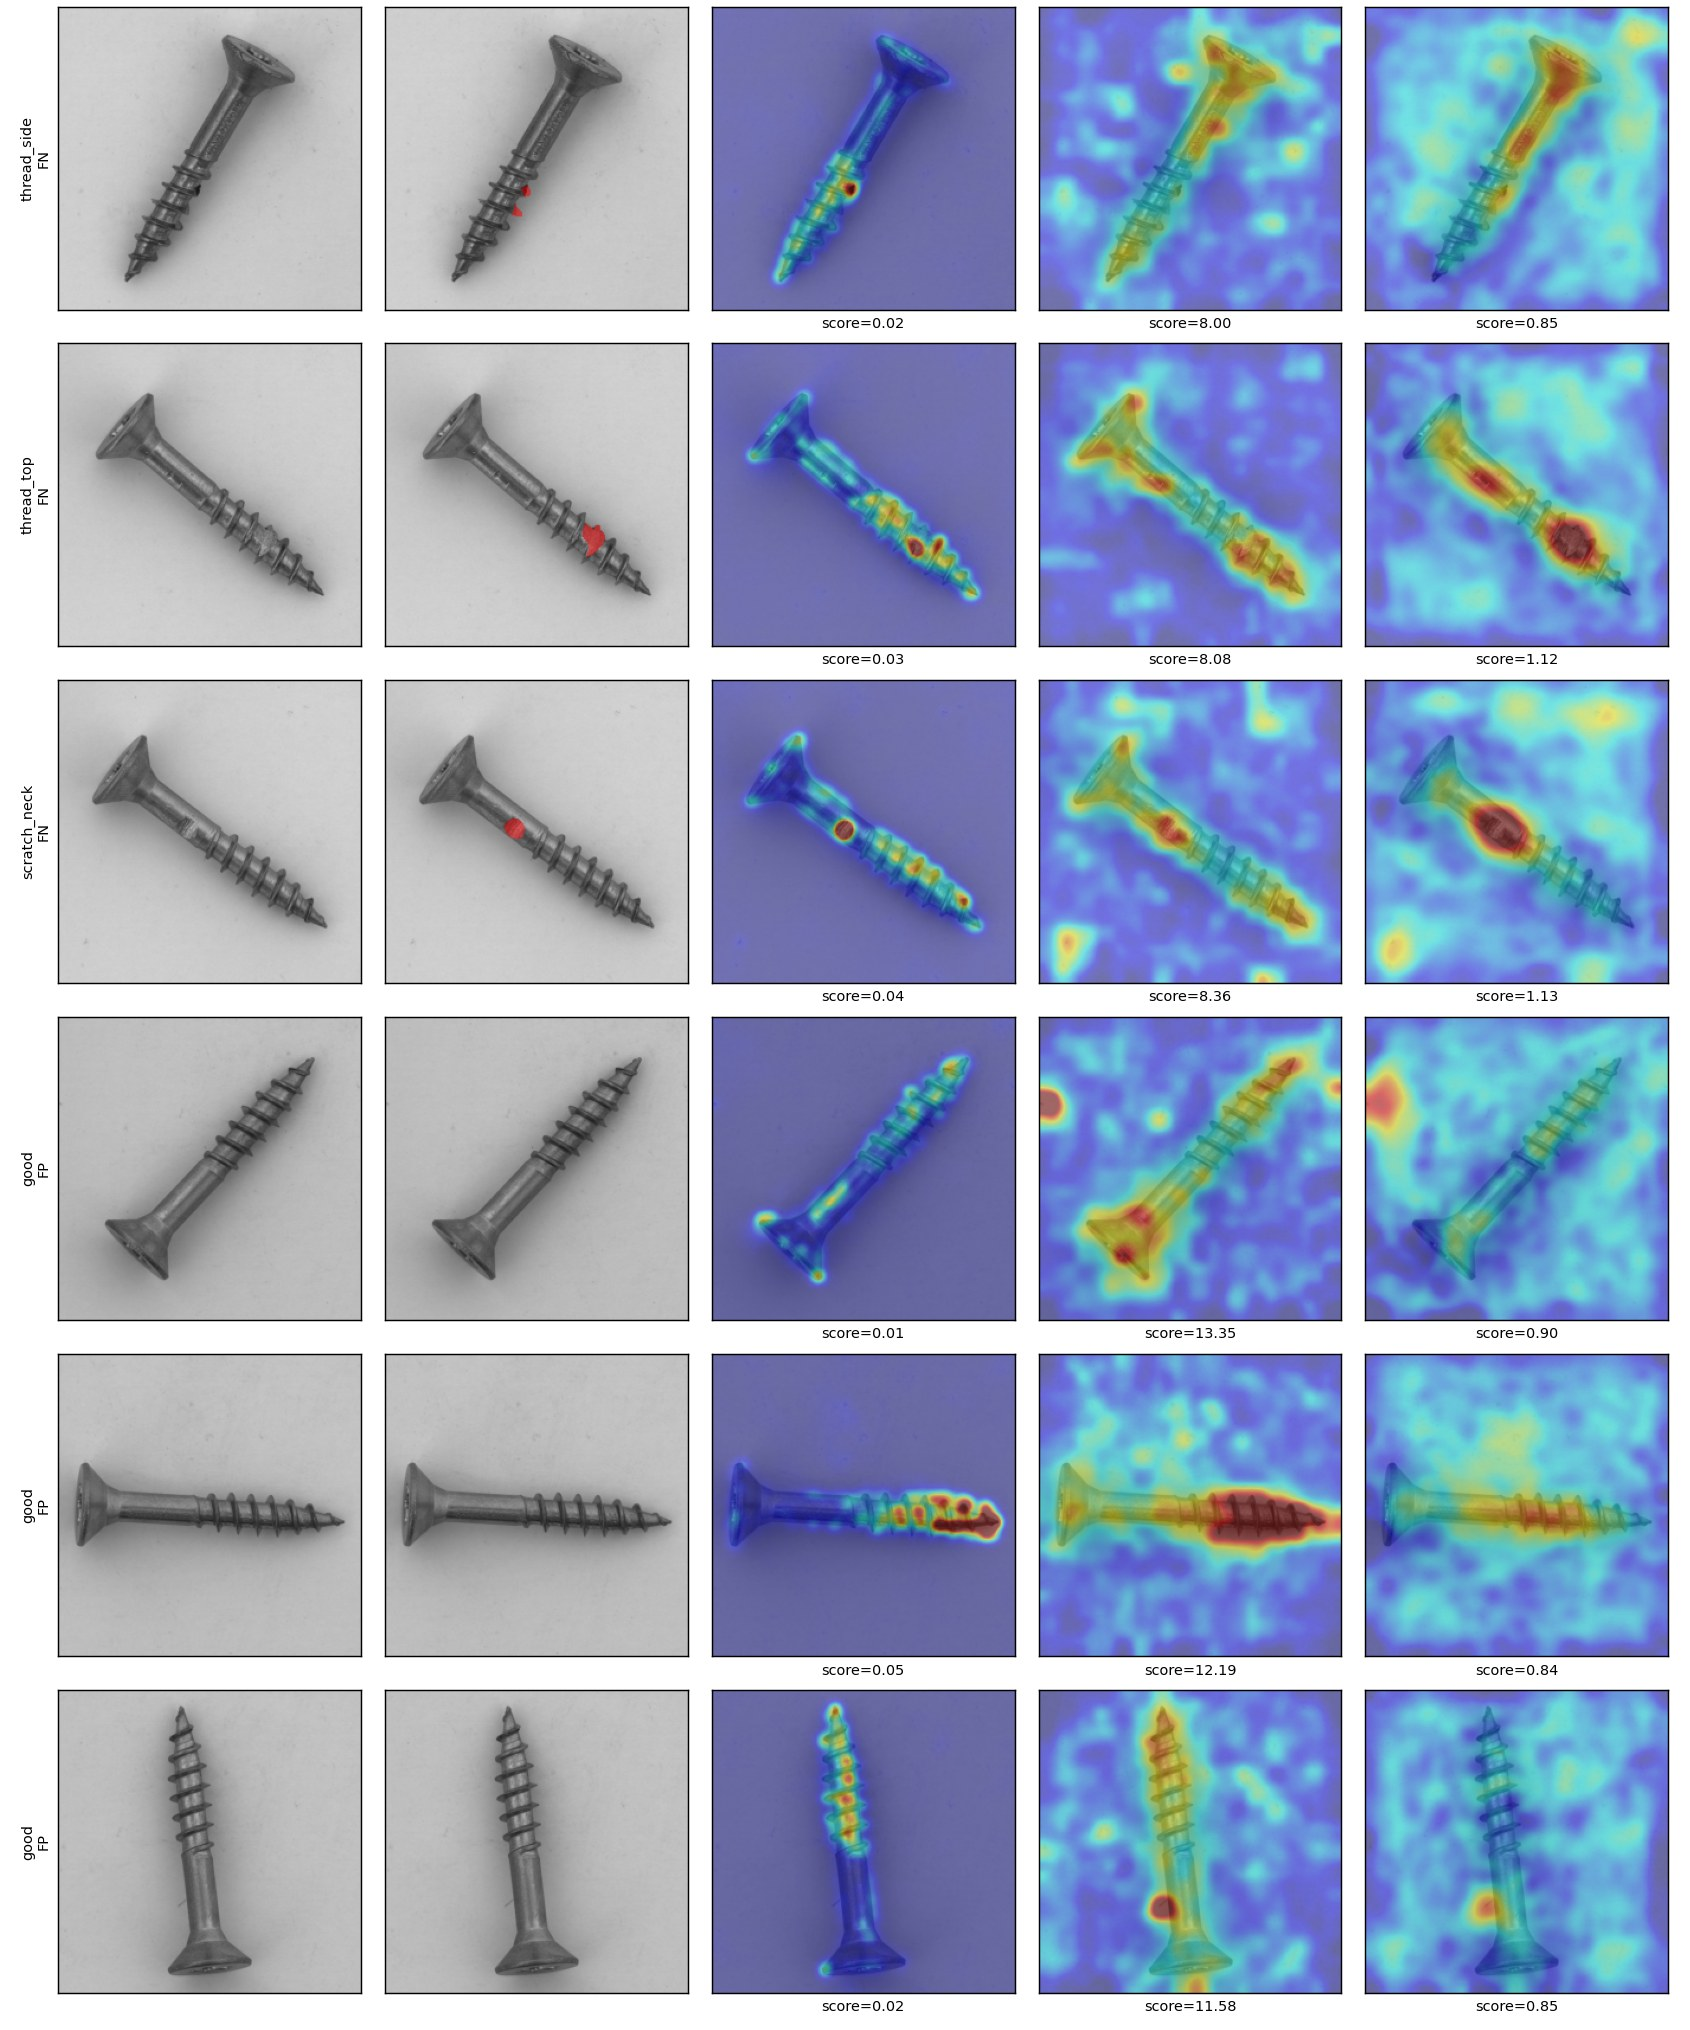
\includegraphics[width=0.7\linewidth]{images/tn/tn5_padim_bao_nham.jpg}
  \caption[Ảnh screw tốt có điểm PaDiM cao nhất]{Những ảnh screw tốt có điểm PaDiM cao nhất (báo nhầm): bản đồ sáng
    dọc cả thân vít}
  \label{fig:tn5-padim}
\end{figure}

\begin{figure}[htbp]
  \centering
  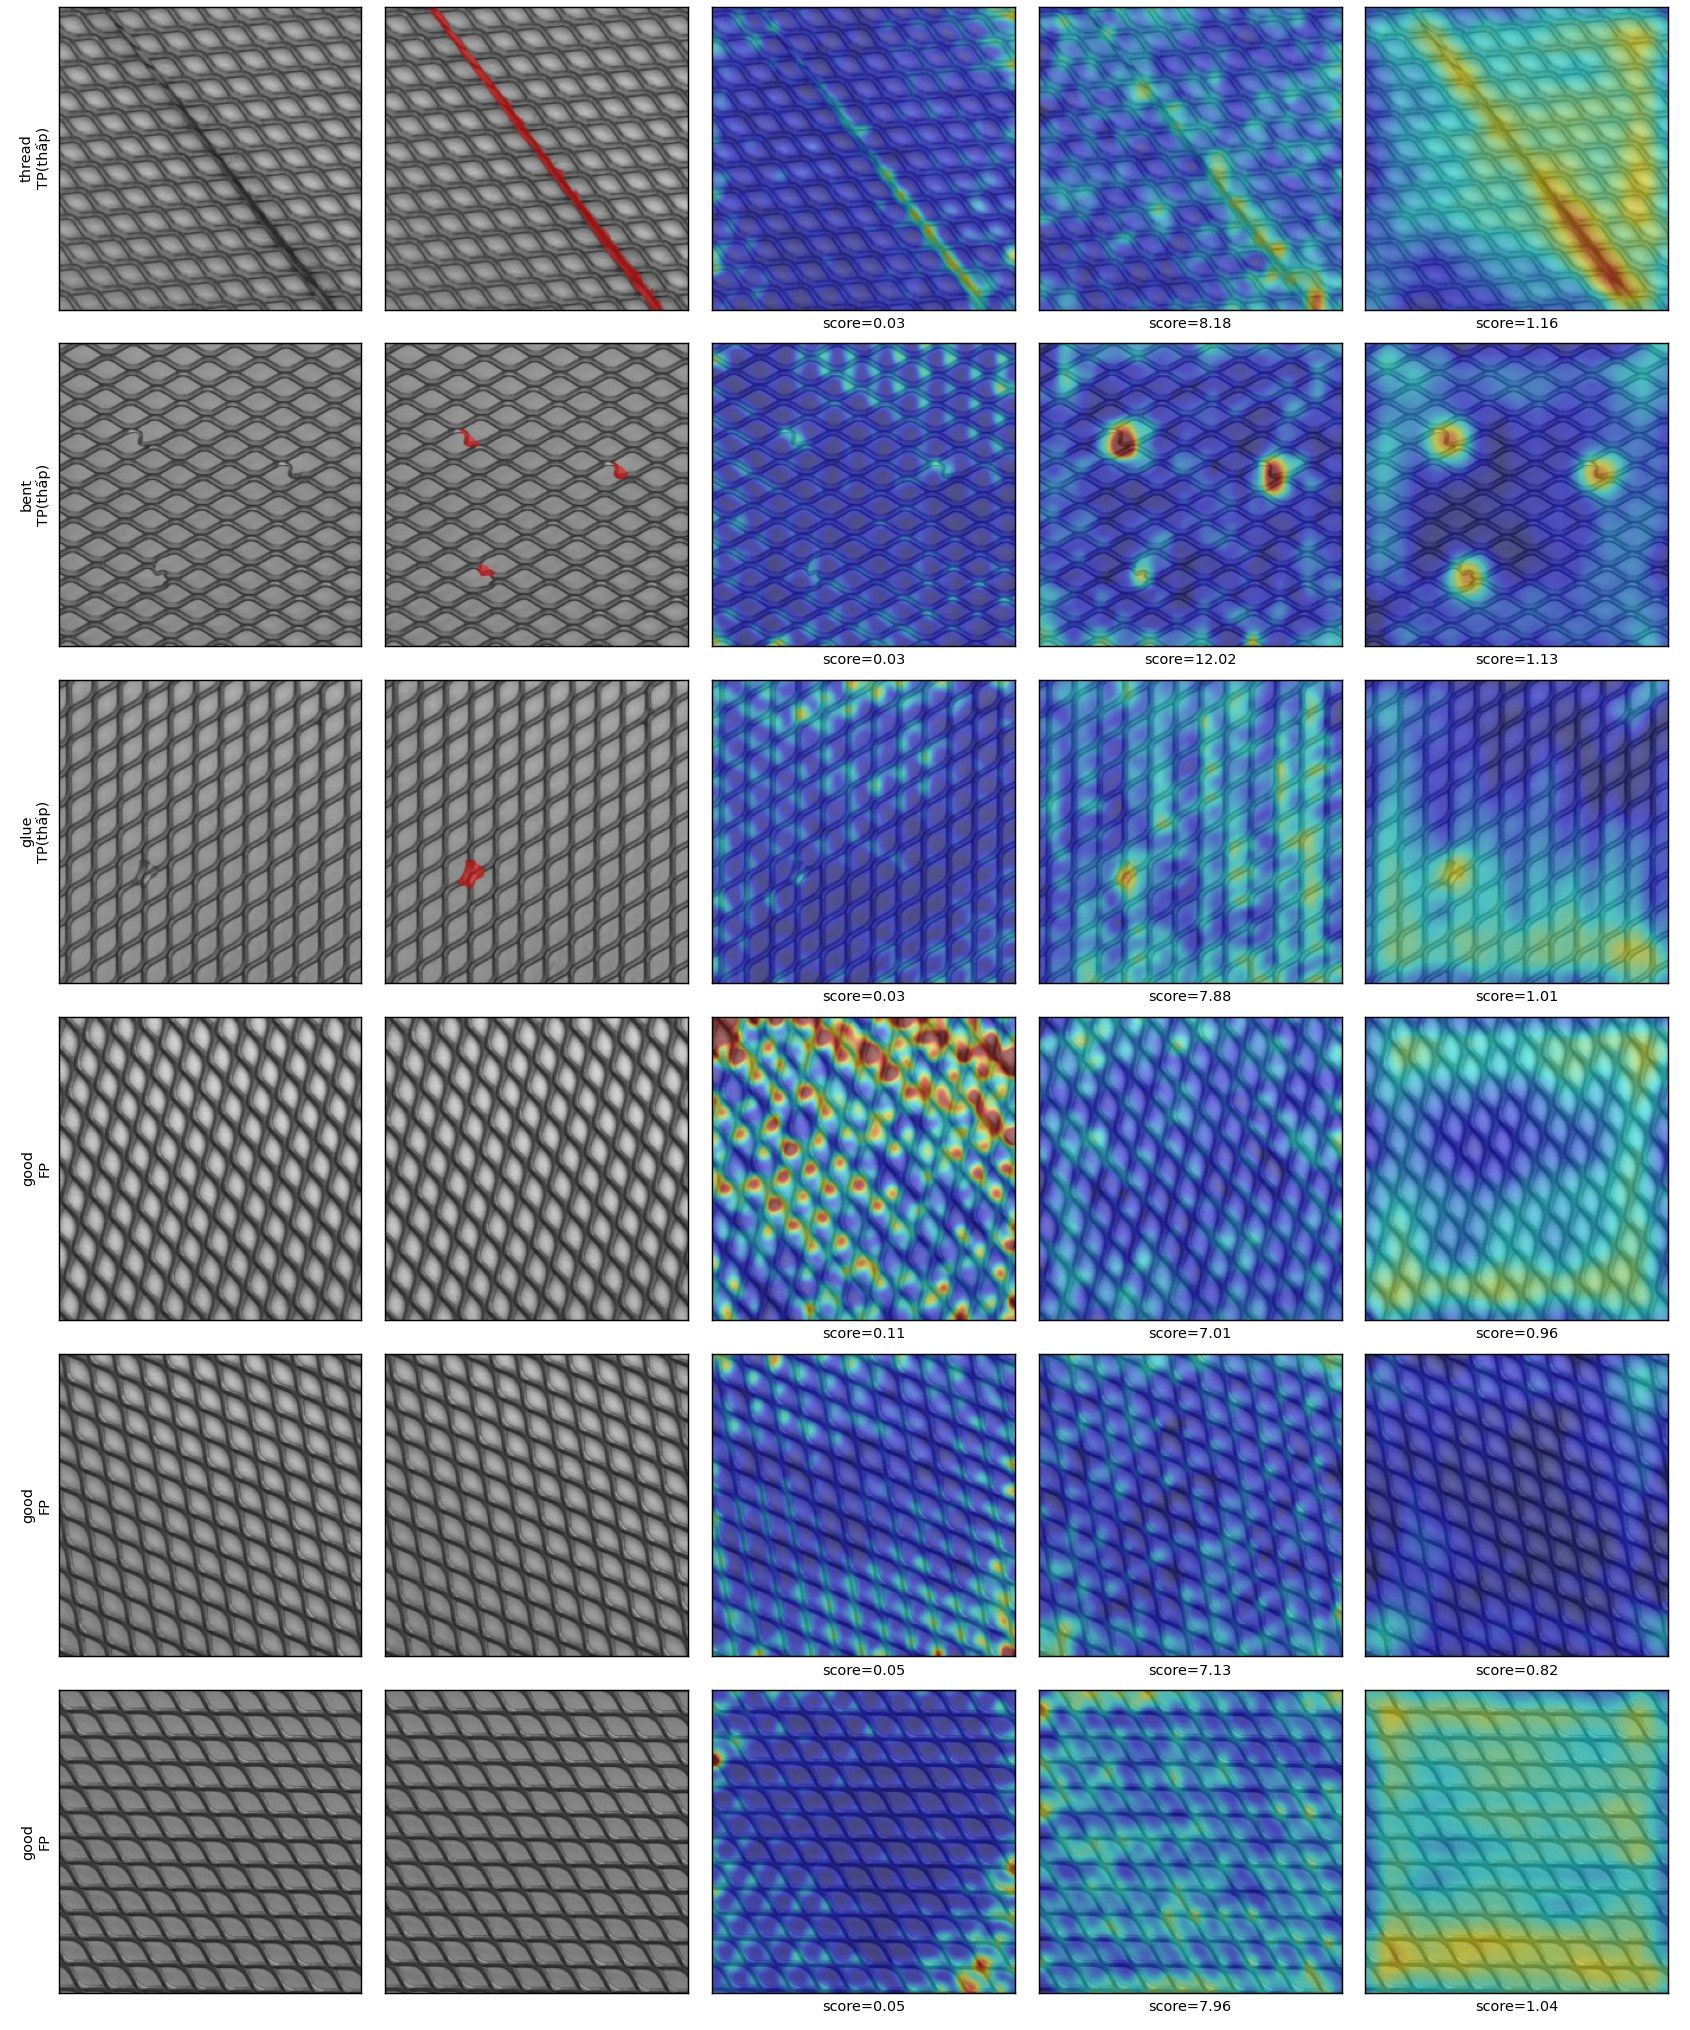
\includegraphics[width=0.7\linewidth]{images/tn/tn5_ae_that_bai.jpg}
  \caption[Các ca thất bại của Autoencoder trên grid]{Các ca thất bại của Autoencoder trên grid: bỏ sót lỗi nhỏ và báo
    nhầm ở vùng sáng}
  \label{fig:tn5-ae}
\end{figure}

Mỗi phương pháp để lại một dấu hiệu nhận biết trên bản đồ. Các ảnh screw tốt bị PaDiM chấm cao nhất đều là vít nằm ở
góc ít gặp, và bản đồ không sáng tại một điểm mà phủ dọc cả thân vít (Hình~\ref{fig:tn5-padim}): mọi vị trí mà thân
vít đi qua đều chỉ được học là nền trắng. Với Autoencoder trên grid, những lỗi nhỏ chỉ cho điểm khoảng 0,03, trong khi
một ảnh tốt có lưới sáng hơn lại đạt 0,11 (Hình~\ref{fig:tn5-ae}); trên transistor, Autoencoder làm sáng các chân kim
loại bóng ngay cả trên ảnh tốt. Cả hai trường hợp là cùng một cơ chế: sai số tái tạo tỷ lệ với độ sáng và độ chi tiết
của vùng ảnh, không tỷ lệ với mức bất thường. Với transistor thiếu linh kiện, PatchCore vẫn xếp ảnh là bất thường
(0,997) nhưng bản đồ yếu và lan rộng, vì vùng thiếu là nền trơn và patch nền trơn có láng giềng trong bộ nhớ (nền ở
các vị trí khác). PaDiM và Autoencoder gắn với vị trí nên định vị vùng thiếu rõ hơn. Đây là mặt trái của việc PatchCore
không dùng thông tin vị trí, cũng chính là lý do nó bền với dịch và xoay ở Thí nghiệm 4.

Các giải thích trên dựa trên bản đồ và AUROC theo kiểu lỗi. Để khẳng định chắc chắn, còn cần ba kiểm tra trực tiếp mà
đề tài chưa thực hiện: hiển thị ảnh dựng lại của Autoencoder để phân biệt ``tái tạo quá tốt'' với ``tái tạo quá kém'';
vẽ phân phối khoảng cách Mahalanobis của patch tốt tại những vị trí PaDiM báo nhầm, để biết patch đó nằm ở đuôi phân
phối hay phân phối tại vị trí đó có nhiều đỉnh; và truy ngược patch gần nhất trong bộ nhớ của PatchCore cho mỗi patch
bị bỏ sót hoặc báo nhầm, để xác nhận vùng thiếu tìm được láng giềng là nền trơn.

\subsection{Thảo luận tổng hợp}
\label{sec:thao-luan}

\begin{table}[htbp]
  \centering
  \caption{Điểm mạnh và điểm yếu của ba phương pháp theo từng tình huống}
  \label{tab:thao-luan}
  \small
  \begin{tabular}{@{}>{\raggedright\arraybackslash}p{3.6cm}>{\raggedright\arraybackslash}p{2.4cm}>{\raggedright\arraybackslash}p{3.3cm}>{\raggedright\arraybackslash}p{3.2cm}l@{}}
    \toprule
    Tình huống & Autoencoder & PaDiM & PatchCore & Mục \\
    \midrule
    Dữ liệu chuẩn, đủ ảnh & Trung bình & Khá & Tốt nhất & \ref{sec:ket-qua-tong-hop} \\
    Dữ liệu huấn luyện lẫn lỗi & Dao động mạnh & Bền nhất & Giảm đều, vẫn cao nhất & \ref{sec:tn1} \\
    Ít ảnh, vật thể cố định (transistor) & Kém & Khá từ 16 ảnh & Tốt từ 4 ảnh & \ref{sec:tn2} \\
    Ít ảnh, vật thể xoay tự do & Thất bại & Thất bại & Thất bại, cần căn chỉnh & \ref{sec:tn2b} \\
    Chuyển sang sản phẩm khác & Thất bại & Thất bại, bị hại khi trộn nguồn & Thất bại, thích nghi nhanh & \ref{sec:tn3} \\
    Độ sáng thay đổi & Rất nhạy & Bền (nhân tạo), nhạy (thật) & Bền, trừ ảnh quá tối & \ref{sec:tn4} \\
    Làm mờ, nhiễu & Bền & Nhạy & Nhạy & \ref{sec:tn4} \\
    Dịch, xoay nhỏ & Nhạy & Nhạy & Bền theo AUPRO, FPR tăng & \ref{sec:tn4} \\
    Lỗi tối trên nền tối, lỗi ren nhỏ & Bỏ sót & Trung bình & Tốt & \ref{sec:tn5} \\
    Vết xước mảnh trên ảnh dài (sheet\_metal) & Kém & Kém & Kém & \ref{sec:tn4} \\
    Định vị lỗi thiếu linh kiện & Tốt & Tốt & Bản đồ lan rộng & \ref{sec:tn5} \\
    \bottomrule
  \end{tabular}
\end{table}

Bảng~\ref{tab:thao-luan} tổng hợp các thí nghiệm. Thứ hạng trên dữ liệu chuẩn, PatchCore rồi PaDiM rồi Autoencoder,
không còn đúng khi điều kiện thay đổi, nhưng cách mỗi phương pháp thất bại phần lớn đoán trước được từ cơ chế. Bốn
quan sát xuyên suốt các thí nghiệm.

Thông tin vị trí là con dao hai lưỡi. PaDiM và Autoencoder gắn với vị trí nên định vị tốt lỗi thiếu linh kiện, nhưng
thất bại khi vật thể xoay hay lệch. PatchCore bỏ qua vị trí nên bền với dịch và xoay, nhưng không biết một vùng nền
trơn lẽ ra phải có linh kiện.

Phát hiện và định vị hỏng theo những cách khác nhau. Dữ liệu bẩn làm hỏng phát hiện nhiều hơn định vị, vì điểm ảnh là
giá trị lớn nhất của bản đồ và rất nhạy với vài patch sai; với ít ảnh, điều này đúng trên screw nhưng ngược lại trên
grid, nơi định vị hỏng trước. Thay đổi vị trí cũng làm hỏng định vị trước. Báo cáo một chỉ số duy nhất sẽ bỏ lỡ một trong hai.

AUROC không đủ để quyết định triển khai. Image-AUROC đo khả năng xếp hạng, còn FPR tại ngưỡng cố định đo điều nhà máy
thực sự gặp. Các trường hợp AUROC giữ nguyên mà FPR lên 100\% ở Thí nghiệm 3 và 4 cho thấy việc đặt lại ngưỡng quan
trọng không kém việc chọn mô hình.

Lối tắt trong dữ liệu có thật và ảnh hưởng tới kết luận. Độ lệch độ sáng giữa ảnh test tốt của screw và các tập khác
đủ để chỉ riêng độ sáng trung bình đạt AUROC 1,0 trên tập kiểm tra. Nó giải thích ít nhất ba kết quả bất thường:
Autoencoder với ít ảnh dưới 0,5, Autoencoder từ transistor sang screw đạt 0,975, và độ nhạy độ sáng cực đoan của
Autoencoder trên screw.
